% ============================================================
%  Chương 4: Thực nghiệm, đánh giá và thảo luận
% ============================================================

Chương này trình bày kết quả thực nghiệm của hệ thống sau khi các thành phần đã được thiết kế và hiện thực ở Chương~\ref{c:phuongphapthuchien}. Nội dung chương được tổ chức theo hai nhóm chính. Nhóm thứ nhất trình bày kết quả huấn luyện và kiểm chứng các mô hình LSTM và PPO. Nhóm thứ hai trình bày các kịch bản đánh giá hệ thống, bao gồm benchmark bộ điều khiển, testcase vận hành LSTM/PPO, kiểm thử pipeline dữ liệu và đo độ trễ suy luận. Các kết quả được diễn giải trong phạm vi mô phỏng và kiểm thử phần mềm, không thay thế cho kiểm định an toàn trên phần cứng gas thực.

\section{Mục tiêu và phạm vi thực nghiệm}
Mục tiêu của phần thực nghiệm là đánh giá toàn bộ hệ thống khi các thành phần IoT, xử lý luồng dữ liệu, dự báo LSTM và điều khiển học tăng cường PPO phối hợp với nhau. Các nội dung đánh giá được tổ chức theo các nội dung sau:

\begin{enumerate}
  \item Đánh giá kết quả huấn luyện mô hình LSTM trong bài toán dự báo rủi ro nồng độ khí gas.
  \item Đánh giá quá trình học và chính sách điều khiển của PPO trong môi trường mô phỏng.
  \item Đánh giá hệ thống qua các kịch bản vận hành, benchmark bộ điều khiển, pipeline dữ liệu và độ trễ xử lý.
\end{enumerate}

Do chưa triển khai kiểm thử an toàn trên phần cứng gas thật, các kết quả trong chương này được hiểu là kết quả kiểm chứng trong môi trường phần mềm có kiểm soát. Dữ liệu công khai được dùng để tham chiếu và kiểm chứng bổ sung cho mô hình LSTM, còn bộ mô phỏng được dùng để tạo nhãn huấn luyện chính, tạo kịch bản vận hành và kiểm thử tích hợp hệ thống.

\section{Môi trường thực nghiệm}

\subsection{Cấu hình phần cứng và phần mềm}

Các thí nghiệm được thực hiện trên máy cá nhân có Docker, đồng thời một số quá trình huấn luyện mô hình được chạy trên Google Colab. Bảng~\ref{tab:env_hardware} mô tả môi trường thực nghiệm chính.

\begingroup
\small
\renewcommand{\arraystretch}{1.25}
\setlength{\LTleft}{0pt}
\setlength{\LTright}{0pt}

\begin{longtable}{
  >{\raggedright\arraybackslash}p{4cm}
  >{\raggedright\arraybackslash}p{\dimexpr\textwidth-4cm-4\tabcolsep\relax}
}
\caption{Cấu hình môi trường thực nghiệm}
\label{tab:env_hardware} \\
\toprule
\textbf{Thành phần} & \textbf{Mô tả} \\
\midrule
\endfirsthead
\toprule
\textbf{Thành phần} & \textbf{Mô tả} \\
\midrule
\endhead
\endfoot
\bottomrule
\endlastfoot

Máy thực nghiệm 
& Laptop/máy trạm cá nhân, Windows 11, Docker Desktop/WSL2 \\

CPU/RAM 
& CPU đa nhân, RAM 16GB \\

Huấn luyện mô hình 
& Môi trường Google Colab CPU và môi trường Python cục bộ \\

Môi trường container 
& Docker Compose \\

Ngôn ngữ 
& Python, TypeScript/JavaScript, PowerShell \\

Message protocol 
& MQTT \\

Message broker 
& Apache Kafka \\

Xử lý luồng dữ liệu 
& Apache Spark Structured Streaming \\

Database 
& InfluxDB cho dữ liệu chuỗi thời gian; PostgreSQL cho lịch sử cảnh báo và hành động \\

Giao diện 
& Bảng điều khiển web, Grafana, Telegram bot \\

\end{longtable}
\endgroup

\section{Dữ liệu thực nghiệm}
\label{sec:dataset_role}
\subsection{Tập dữ liệu kiểm chứng}
\label{ssec:validated_dataset}
Tập dữ liệu công khai đầu tiên được khảo sát là \textit{UCI Gas Sensor Array Under Dynamic Gas Mixtures}. Đây là tập dữ liệu chuỗi thời gian đa biến, được thu từ 16 cảm biến khi tiếp xúc với các hỗn hợp khí thay đổi động theo thời gian. Theo mô tả của UCI Machine Learning Repository, dữ liệu được thu liên tục với tần số 100\,Hz, gồm hai hỗn hợp khí chính: Ethylene--Methane và Ethylene--CO trong không khí~\cite{uci_gas_dynamic}.

UCI được dùng như nguồn tham chiếu về đặc tính chuỗi thời gian của cảm biến khí: tín hiệu có quán tính, nhiễu và thay đổi theo quá trình phơi nhiễm khí. Tuy nhiên, tập này không cùng cấu trúc dữ liệu với luồng triển khai, không chứa LPG dân dụng, nhiệt độ--độ ẩm theo cách hệ thống sử dụng và không có nhãn hành động điều khiển. Vì vậy, UCI không được dùng làm dữ liệu huấn luyện khi hệ thống vận hành, mà được dùng để củng cố cơ sở lựa chọn hướng dự báo chuỗi thời gian.

\begingroup
\footnotesize
\renewcommand{\arraystretch}{1.35}
\setlength{\tabcolsep}{3pt}
\setlength{\LTleft}{0pt}
\setlength{\LTright}{0pt}

\begin{longtable}{
  >{\raggedright\arraybackslash}p{3.0cm}
  >{\centering\arraybackslash}p{2.3cm}
  >{\centering\arraybackslash}p{1.8cm}
  >{\raggedright\arraybackslash}p{\dimexpr\textwidth-7.1cm-8\tabcolsep\relax}
}
\caption{Mô tả các file dữ liệu trong tập UCI Gas Sensor Array Under Dynamic Gas Mixtures}
\label{tab:uci_gas_dataset} \\
\toprule
\textbf{File dữ liệu} 
& \textbf{Số điểm dữ liệu} 
& \textbf{Số thuộc tính} 
& \textbf{Mô tả thuộc tính} \\
\midrule
\endfirsthead
\toprule
\textbf{File dữ liệu} 
& \textbf{Số điểm dữ liệu} 
& \textbf{Số thuộc tính} 
& \textbf{Mô tả thuộc tính} \\
\midrule
\endhead
\endfoot
\bottomrule
\endlastfoot

\makecell[l]{\texttt{ethylene\_}\\\texttt{methane.txt}}
& 4{,}208{,}261
& 19
& Thời gian, nồng độ Methane, nồng độ Ethylene và 16 kênh tín hiệu cảm biến. \\

\makecell[l]{\texttt{ethylene\_}\\\texttt{CO.txt}}
& 4{,}178{,}504
& 19
& Thời gian, nồng độ CO, nồng độ Ethylene và 16 kênh tín hiệu cảm biến. \\

\end{longtable}
\endgroup

Hình~\ref{fig:uci_dataset_histogram} bổ sung góc nhìn trực quan về quy mô hai file dữ liệu trong tập UCI. Hai file có số điểm dữ liệu xấp xỉ nhau, đều trên 4 triệu mẫu, cho thấy đây là tập dữ liệu chuỗi thời gian đủ dài để tham chiếu đặc tính động của cảm biến khí. Tuy nhiên, histogram này chỉ dùng để mô tả quy mô tập kiểm chứng, không hàm ý UCI được dùng trực tiếp làm dữ liệu huấn luyện vận hành.

\Needspace{0.45\textheight}
\begin{center}
  
\includegraphics[width=0.92\linewidth]{exp/uci_dataset_histogram.png}
  \captionof{figure}{Histogram quy mô hai file dữ liệu trong tập UCI theo số điểm dữ liệu.}
  \label{fig:uci_dataset_histogram}
\end{center}

Về kết quả huấn luyện trên UCI, khóa luận không trình bày một bảng đánh giá riêng vì mô hình LSTM hiện tại không được huấn luyện trực tiếp trên tập này. UCI chứa Methane/Ethylene/CO và 16 kênh cảm biến, trong khi pipeline của hệ thống dùng \texttt{gas\_ppm}, temperature, humidity và nhãn sự kiện ``vượt ngưỡng trong 5 phút tới''. Nếu ép UCI thành bài toán dự báo nồng độ CO/Methane liên tục thì đó là một thí nghiệm hồi quy khác, cần đánh giá bằng MAE/RMSE/R\textsuperscript{2} theo đơn vị khí tương ứng, không so sánh trực tiếp với đầu ra \texttt{predicted\_risk\_5min}. Vì vậy, UCI chỉ được dùng làm dataset tham chiếu để giải thích đặc tính chuỗi thời gian của cảm biến khí.

Ngoài UCI dataset, đề tài sử dụng thêm tập \textit{Environmental Sensor Telemetry Data} từ Kaggle để kiểm chứng bổ sung trên dữ liệu cảm biến IoT thực~\cite{stafford2020envsensor}. Tập dữ liệu này chứa tín hiệu LPG, CO, smoke, nhiệt độ và độ ẩm từ các thiết bị IoT sử dụng Raspberry Pi, gần với cấu trúc đầu vào của LSTM hơn UCI. Tuy nhiên, dữ liệu không cung cấp nhãn rò rỉ LPG thật, do đó nhãn dương chỉ được xây dựng theo quy tắc proxy dựa trên phân vị cao của tín hiệu LPG. Vì vậy, kết quả trên Kaggle chỉ dùng để kiểm tra sơ bộ khả năng học xu hướng của kiến trúc LSTM trên dữ liệu cảm biến thực, không dùng để kết luận an toàn.

\begingroup
\footnotesize
\renewcommand{\arraystretch}{1.35}
\setlength{\tabcolsep}{4pt}
\setlength{\LTleft}{0pt}
\setlength{\LTright}{0pt}

\begin{longtable}{
  >{\raggedright\arraybackslash}p{3.2cm}
  >{\centering\arraybackslash}p{2.4cm}
  >{\centering\arraybackslash}p{2.0cm}
  >{\raggedright\arraybackslash}p{\dimexpr\textwidth-7.6cm-8\tabcolsep\relax}
}
\caption{Mô tả tập dữ liệu Environmental Sensor Telemetry Data từ Kaggle}
\label{tab:kaggle_env_sensor_dataset} \\
\toprule
\textbf{Tên tập dữ liệu} 
& \textbf{Số điểm dữ liệu} 
& \textbf{Số thuộc tính} 
& \textbf{Mô tả thuộc tính} \\
\midrule
\endfirsthead
\toprule
\textbf{Tên tập dữ liệu} 
& \textbf{Số điểm dữ liệu} 
& \textbf{Số thuộc tính} 
& \textbf{Mô tả thuộc tính} \\
\midrule
\endhead
\endfoot
\bottomrule
\endlastfoot

\makecell[l]{\textit{Environmental}\\\textit{Sensor Telemetry}\\\textit{Data}}
& 405{,}184
& 9
& Timestamp, \texttt{device\_id}, CO, humidity, light, LPG, motion, smoke, temperature. \\

\end{longtable}
\endgroup

Hình~\ref{fig:kaggle_dataset_histogram} mô tả số dòng thô của Kaggle dataset và phân bố các cửa sổ chuỗi thời gian sau khi gán nhãn sự kiện tương lai. Phần màu vàng biểu diễn các cửa sổ dương theo nhãn proxy, tức là cửa sổ hiện tại dẫn đến tín hiệu LPG cao trong chân trời dự báo. Tỷ lệ dương trên tập kiểm thử chỉ khoảng 1{,}31\%, vì vậy khi quan sát tầng cảnh báo sau ngưỡng trên Kaggle cần xem Recall, Precision và ma trận nhầm lẫn thay vì chỉ nhìn Accuracy.

\Needspace{0.45\textheight}
\begin{center}
  
\includegraphics[width=0.95\linewidth]{exp/kaggle_dataset_histogram.png}
  \captionof{figure}{Histogram dữ liệu Kaggle sau khi chuyển thành cửa sổ chuỗi thời gian và nhãn sự kiện.}
  \label{fig:kaggle_dataset_histogram}
\end{center}

\subsection{Dữ liệu bộ mô phỏng}

Trong phạm vi đề tài, bộ mô phỏng được sử dụng để sinh dữ liệu mô phỏng và tạo môi trường thực nghiệm có kiểm soát. Dữ liệu mô phỏng không được xem là tập dữ liệu đã được chứng thực như các tập dữ liệu công khai UCI/Kaggle, mà là dữ liệu tổng hợp được sinh theo các quy tắc và kịch bản đã định nghĩa trước. Vai trò chính của bộ mô phỏng là:

\begin{itemize}
  \item Tạo dữ liệu huấn luyện có nhãn cho mô hình LSTM trong môi trường mô phỏng. Nhãn được sinh theo quy tắc dự báo, tức là kiểm tra xem nồng độ khí có vượt ngưỡng trong 5 phút tiếp theo hay không.
  
  \item Cung cấp môi trường tương tác cho bộ điều khiển PPO. Đây là vai trò quan trọng vì học tăng cường cần tác nhân thực hiện hành động và nhận phản hồi từ môi trường, trong khi các dataset log tĩnh như UCI/Kaggle không phản hồi lại hành động điều khiển.
  
  \item Tạo các testcase có kiểm soát như trạng thái bình thường, rò rỉ chậm, rò rỉ nhanh và thông gió để benchmark các bộ điều khiển.
  
  \item Kiểm thử luồng xử lý đầu cuối vì bộ mô phỏng gửi dữ liệu theo cùng cấu trúc JSON với thiết bị ESP32 dự kiến.
\end{itemize}

Nói cách khác, UCI/Kaggle nằm ở khối tham chiếu và kiểm chứng bổ sung trong giai đoạn phát triển mô hình, còn bộ mô phỏng nằm ở khối dữ liệu huấn luyện, bộ kiểm thử và môi trường tương tác cho PPO. Khi hệ thống vận hành, luồng xử lý không phân biệt dữ liệu đến từ ESP32 thật hay bộ mô phỏng, miễn là bản tin có cùng cấu trúc dữ liệu.

Hình~\ref{fig:sim_dataset_histogram} trực quan hóa phân bố dữ liệu mô phỏng được dùng để huấn luyện LSTM. Biểu đồ bên trái cho thấy phần lớn mẫu nằm ở vùng nền thấp, trong khi các mẫu vượt ngưỡng 1000\,ppm xuất hiện ít hơn và chủ yếu thuộc các pha rò rỉ. Biểu đồ bên phải cho thấy phân bố nhãn dự báo sự kiện: nhãn dương được gán khi cửa sổ hiện tại dẫn đến nguy cơ vượt ngưỡng trong 5 phút tiếp theo. Tỷ lệ mẫu dương khoảng 27{,}4\% cho thấy dữ liệu có mất cân bằng nhưng chưa đến mức cực đoan, vì vậy các chỉ số cảnh báo sau ngưỡng như Precision, Recall và F1-score cần được xem cùng Accuracy.

\Needspace{0.45\textheight}
\begin{center}
  
\includegraphics[width=1\linewidth]{exp/sim_dataset_histogram.png}
  \captionof{figure}{Histogram dữ liệu mô phỏng và phân bố nhãn dự báo sự kiện của LSTM.}
  \label{fig:sim_dataset_histogram}
\end{center}

\begingroup
\scriptsize
\renewcommand{\arraystretch}{1.18}
\setlength{\tabcolsep}{2.5pt}
\setlength{\LTleft}{0pt}
\setlength{\LTright}{0pt}

\begin{longtable}{
  >{\raggedright\arraybackslash}p{3.0cm}
  >{\raggedright\arraybackslash}p{3.5cm}
  >{\raggedright\arraybackslash}p{\dimexpr\textwidth-6.5cm-6\tabcolsep\relax}
}
\caption{Các trường dữ liệu chính trong thực nghiệm}
\label{tab:data_fields} \\
\toprule
\textbf{Trường dữ liệu} 
& \textbf{Ý nghĩa} 
& \textbf{Vai trò trong mô hình/hệ thống} \\
\midrule
\endfirsthead
\toprule
\textbf{Trường dữ liệu} 
& \textbf{Ý nghĩa} 
& \textbf{Vai trò trong mô hình/hệ thống} \\
\midrule
\endhead
\endfoot
\bottomrule
\endlastfoot

\texttt{device\_id} 
& Định danh thiết bị nguồn 
& Metadata, dùng để lọc dữ liệu theo thiết bị hoặc testcase. \\

\texttt{event\_ts} 
& Thời điểm phát sinh bản tin 
& Sắp xếp dữ liệu theo chuỗi thời gian và hỗ trợ tính độ trễ xử lý. \\

\texttt{gas\_ppm} 
& Nồng độ khí gas 
& Đầu vào của mô hình LSTM và là thành phần trạng thái của PPO. \\

\makecell[l]{\texttt{temperature\_}\\\texttt{c}}
& Nhiệt độ môi trường 
& Đầu vào cho LSTM và PPO để bổ sung ngữ cảnh môi trường. \\

\makecell[l]{\texttt{humidity\_}\\\texttt{percent}}
& Độ ẩm môi trường 
& Đầu vào cho LSTM và PPO để bổ sung ngữ cảnh môi trường. \\

\makecell[l]{\texttt{predicted\_risk}\\\texttt{\_5min}}
& Xác suất nguy hiểm trong 5 phút tiếp theo 
& Đầu ra của bộ dự báo LSTM và được dùng làm một thành phần đầu vào cho PPO. \\

\texttt{rl\_action} 
& Hành động điều khiển 
& Đầu ra của PPO, dùng để hiển thị trên bảng điều khiển và gửi sang Kafka action topic. \\

\end{longtable}
\endgroup

\section{Tiêu chí đánh giá}

Các tiêu chí đánh giá được lựa chọn nhằm phản ánh ba khía cạnh chính của hệ thống: khả năng dự báo của mô hình LSTM, hiệu quả điều khiển của PPO và độ tin cậy của pipeline dữ liệu. Bảng~\ref{tab:metrics} tổng hợp các tiêu chí được sử dụng trong quá trình thực nghiệm. Các công thức và ý nghĩa được trình bày tại đây để tránh lặp lại trong các phần đánh giá riêng phía sau.

\begingroup
\footnotesize
\renewcommand{\arraystretch}{1.28}
\setlength{\tabcolsep}{2pt}

% Kéo rộng bảng nhẹ sang hai bên để cột Ý nghĩa đỡ xuống dòng
\setlength{\LTleft}{-0.35cm}
\setlength{\LTright}{-0.35cm}

\begin{longtable}{
  >{\centering\arraybackslash}p{1.6cm}
  >{\raggedright\arraybackslash}p{3.0cm}
  >{\raggedright\arraybackslash}p{3.6cm}
  >{\raggedright\arraybackslash}p{\dimexpr\textwidth+0.7cm-1.6cm-3.0cm-3.6cm-8\tabcolsep\relax}
}
\caption{Tổng hợp các tiêu chí đánh giá}
\label{tab:metrics} \\
\toprule
\textbf{Nhóm} 
& \textbf{Tiêu chí} 
& \textbf{Công thức / cách tính} 
& \textbf{Ý nghĩa} \\
\midrule
\endfirsthead

% Không lặp lại header nếu bảng bị cắt sang trang mới
\endhead

% Không thêm dòng "Còn tiếp ở trang sau"
\endfoot

\bottomrule
\endlastfoot

\multirow{7}{*}{\textbf{LSTM}}
& \makecell[l]{\texttt{predicted\_risk}\\\texttt{\_5min}}
& $p_{5min} \in [0,1]$
& Chuỗi xác suất rủi ro do LSTM sinh ra theo từng cửa sổ trượt. Đây là đầu ra chính của bài toán time-series forecasting và được dùng làm đầu vào cho bộ điều khiển PPO. \\

& Binary cross-entropy
& $\displaystyle -\frac{1}{n}\sum_{i=1}^{n}\bigl[y_i\log(p_i)+(1-y_i)\log(1-p_i)\bigr]$
& Hàm mất mát huấn luyện cho bài toán dự báo sự kiện tương lai. Chỉ số này làm việc trực tiếp với xác suất $p_i$, chưa cần chuyển thành nhãn cứng. \\

& MAE sự kiện
& $\displaystyle \frac{1}{n}\sum_{i=1}^{n}|y_i-p_i|$
& Sai số tuyệt đối trung bình giữa nhãn sự kiện tương lai và xác suất dự báo. Tiêu chí này đo lỗi của sự kiện 0/1, không phải sai số nồng độ khí theo ppm. \\

& RMSE sự kiện
& $\displaystyle \sqrt{\frac{1}{n}\sum_{i=1}^{n}(y_i-p_i)^2}$
& Sai số bình phương trung bình trên xác suất dự báo sự kiện. Nếu mô hình đổi sang dự báo trực tiếp \texttt{gas\_ppm}, khi đó mới diễn giải RMSE theo đơn vị ppm. \\

& \makecell[l]{Confusion matrix\\(sau ngưỡng)}
& $\hat{y}_i=\mathbf{1}[p_i\geq\theta]$
& Chỉ dùng để kiểm tra tầng cảnh báo sau khi chuỗi xác suất được ngưỡng hóa, không phải metric chính của tầng time-series forecasting. \\

& \makecell[l]{Precision, Recall,\\F1-score}
& $\displaystyle P=\frac{TP}{TP+FP},\quad R=\frac{TP}{TP+FN}$
& Đánh giá chất lượng cảnh báo nhị phân sau ngưỡng. Recall quan trọng trong bài toán an toàn vì liên quan đến nguy cơ bỏ sót rò rỉ. \\

& Accuracy sau ngưỡng
& $\displaystyle \frac{TP+TN}{TP+TN+FP+FN}$
& Tỷ lệ quyết định cảnh báo đúng sau ngưỡng. Chỉ số này chỉ dùng kèm Precision/Recall vì dữ liệu có thể mất cân bằng. \\

\midrule

\multirow{5}{*}{\textbf{PPO}}
& \texttt{miss\_rate}
& $\displaystyle \frac{N_{\mathrm{miss}}}{N_{\mathrm{episode}}}$
& Tỷ lệ episode mà hệ thống để nồng độ khí chạm hoặc vượt ngưỡng nguy hiểm. Giá trị càng thấp cho thấy chính sách điều khiển càng an toàn. \\

& \texttt{peak\_gas}
& $\displaystyle \max_t gas_t$
& Nồng độ khí lớn nhất trong một episode. Chỉ số này phản ánh mức độ nghiêm trọng của tình huống sau khi bộ điều khiển can thiệp. \\

& Lead time
& $\displaystyle t_{\mathrm{threshold}} - t_{\mathrm{alert}}$
& Khoảng thời gian cảnh báo sớm trước khi nồng độ khí đạt ngưỡng nguy hiểm. Lead time càng lớn thì hệ thống càng có nhiều thời gian để phản ứng. \\

& \texttt{alarms/hour}
& $\displaystyle \frac{N_{\mathrm{alarm}}}{T_{\mathrm{hour}}}$
& Số cảnh báo trung bình trong một giờ. Chỉ số này dùng để đánh giá mức độ cảnh báo quá nhiều hoặc gây phiền nhiễu cho người dùng. \\

& Tỷ lệ can thiệp
& $\displaystyle \frac{N_{\mathrm{action}}}{N_{\mathrm{step}}}$
& Tỷ lệ bước thời gian mà bộ điều khiển chọn hành động can thiệp như cảnh báo, bật quạt hoặc đóng van. Chỉ số này phản ánh mức độ điều khiển quá mức. \\

\midrule

\multirow{4}{*}{\textbf{Pipeline}}
& Tỷ lệ truyền thành công
& $\displaystyle \frac{N_{\mathrm{received}}}{N_{\mathrm{sent}}}$
& Tỷ lệ bản tin được nhận và xử lý thành công so với số bản tin được gửi vào hệ thống. Tiêu chí này kiểm tra dữ liệu có đi qua đầy đủ các thành phần chính hay không. \\

& Throughput
& $\displaystyle \frac{N_{\mathrm{message}}}{T}$
& Số bản tin hệ thống xử lý được trong một đơn vị thời gian. Chỉ số này phản ánh khả năng đáp ứng khi dữ liệu tăng nhanh hoặc xuất hiện burst. \\

& Latency
& $\displaystyle t_{\mathrm{output}} - t_{\mathrm{input}}$
& Thời gian từ khi bản tin đi vào pipeline đến khi có kết quả xử lý hoặc hành động đầu ra. Độ trễ càng thấp thì hệ thống càng gần thời gian thực. \\

& Tỷ lệ phục hồi
& $\displaystyle \frac{N_{\mathrm{recovered}}}{N_{\mathrm{error}}}$
& Tỷ lệ trường hợp lỗi mà hệ thống vẫn tiếp tục chạy hoặc xử lý được sau khi gặp bản tin sai định dạng, lỗi tạm thời hoặc sự cố thành phần. \\

\end{longtable}
\endgroup

Trong đó, $p_i=p_{5min}(t_i)$ là xác suất rủi ro trong 5 phút tiếp theo tại cửa sổ thứ $i$, $y_i$ là nhãn sự kiện tương lai và $\hat{y}_i=\mathbf{1}[p_i\geq\theta]$ chỉ là quyết định cảnh báo sau ngưỡng. $TP$ là số mẫu nguy hiểm được cảnh báo đúng, $FP$ là số mẫu an toàn bị cảnh báo nhầm, $TN$ là số mẫu an toàn được dự đoán đúng và $FN$ là số mẫu nguy hiểm bị bỏ sót. Ký hiệu $N_{\mathrm{miss}}$ là số episode vượt ngưỡng nguy hiểm, $N_{\mathrm{episode}}$ là tổng số episode đánh giá, $N_{\mathrm{alarm}}$ là số lần cảnh báo, $T_{\mathrm{hour}}$ là thời gian đánh giá tính theo giờ, $N_{\mathrm{sent}}$ và $N_{\mathrm{received}}$ lần lượt là số bản tin gửi vào và nhận được ở đầu ra của pipeline.

\section{Kết quả huấn luyện mô hình}
\label{sec:model_training_results}

Phần này trình bày kết quả huấn luyện và kiểm chứng hai mô hình chính của hệ thống: bộ dự báo LSTM và bộ điều khiển PPO. LSTM được đánh giá theo khả năng dự báo sự kiện nguy hiểm trong tương lai gần, trong khi PPO được đánh giá thông qua quá trình học chính sách điều khiển trong môi trường mô phỏng.

\subsection{Kết quả huấn luyện và kiểm chứng LSTM}
\label{sec:lstm_eval}

\subsubsection{Bài toán và cấu hình mô hình}

Mô hình LSTM được sử dụng để dự báo nguy cơ nồng độ khí vượt ngưỡng trong tương lai gần. Đầu vào của mô hình là một cửa sổ chuỗi thời gian gồm 60 mẫu gần nhất, với ba đặc trưng cảm biến chính:

\[
X_t = [gas\_ppm, temperature\_c, humidity\_percent]_{t-59:t}.
\]

Đầu ra của mô hình là một giá trị xác suất trong khoảng $[0,1]$, ký hiệu là $p_{5min}$. Giá trị này biểu diễn khả năng nồng độ khí sẽ vượt ngưỡng 1000\,ppm trong 5 phút tiếp theo:

\[
p_{5min} = P\left(\max_{t < \tau \leq t+300} gas_\tau > 1000\,ppm\right).
\]

Khi hệ thống chạy liên tục, mỗi cửa sổ trượt sinh ra một giá trị $p_{5min}(t)$, tạo thành chuỗi \texttt{predicted\_risk\_5min} theo thời gian. Như vậy, LSTM không chỉ phân loại trạng thái hiện tại của môi trường, mà thực hiện bài toán \emph{dự báo nguy cơ trong tương lai}. Classification chỉ xuất hiện ở bước sau, khi chuỗi xác suất này được so với một ngưỡng để tạo cảnh báo nhị phân.

\subsubsection{Tiêu chí đánh giá LSTM}

Đầu ra của LSTM là xác suất của một sự kiện tương lai, không phải nhãn trạng thái hiện tại. Vì vậy, phần đánh giá được tách thành hai tầng. Ở tầng time-series forecasting, chuỗi $p_{5min}(t)$ thể hiện xu hướng rủi ro theo thời gian và được đánh giá bằng loss/MAE/RMSE trên biến sự kiện tương lai. Ở tầng alert/classification, sau khi chọn ngưỡng quyết định, xác suất này mới được chuyển thành cảnh báo nhị phân để tính Accuracy, Precision, Recall, F1-score và confusion matrix. Nói cách khác, confusion matrix không thay thế đánh giá time-series; nó chỉ trả lời câu hỏi nếu dùng ngưỡng $\theta$ thì hệ thống cảnh báo đúng/sai như thế nào. Nếu đổi mục tiêu thành dự báo trực tiếp giá trị nồng độ khí liên tục, khi đó mới cần MAE/RMSE theo đơn vị ppm.

\Needspace{0.42\textheight}
\begin{center}
  
\includegraphics[width=0.95\linewidth]{exp/lstm_evaluation_flow.png}
  \captionof{figure}{Sơ đồ tách tầng đánh giá LSTM giữa time-series forecasting và alert/classification sau ngưỡng.}
  \label{fig:lstm_evaluation_flow}
\end{center}

\subsubsection{Kết quả trên trace mô phỏng}

Trace mô phỏng được sử dụng để đánh giá khả năng dự báo sự kiện trong môi trường có nhãn thật rõ ràng. Kết quả từ file \texttt{lstm\_metrics.json} được tổng hợp trong Bảng~\ref{tab:lstm_metrics}.

\begingroup
\small
\renewcommand{\arraystretch}{1.25}
\setlength{\tabcolsep}{5pt}
\setlength{\LTleft}{\fill}
\setlength{\LTright}{\fill}

\begin{longtable}{lc}
\caption{Kết quả đánh giá LSTM trên tập kiểm thử mô phỏng}
\label{tab:lstm_metrics} \\
\toprule
\textbf{Chỉ số} & \textbf{Giá trị} \\
\midrule
\endfirsthead
\toprule
\textbf{Chỉ số} & \textbf{Giá trị} \\
\midrule
\endhead
\endfoot
\bottomrule
\endlastfoot
Train windows & 22{,}752 \\
Test windows & 5{,}688 \\
Input window & 60 mẫu \\
Forecast horizon & 300\,s \\
Epochs & 20 \\
Positive rate toàn bộ & 27{,}43\% \\
Accuracy sau ngưỡng & 90{,}51\% \\
Precision sau ngưỡng & 100{,}00\% \\
Recall sau ngưỡng & 55{,}15\% \\
F1-score sau ngưỡng & 71{,}09\% \\
TP / FP / TN / FN & 664 / 0 / 4{,}484 / 540 \\
\end{longtable}
\endgroup

Trong huấn luyện LSTM, một \textit{epoch} là một lượt mô hình đi qua toàn bộ tập train một lần. Số epoch không phải đầu ra của hệ thống, mà là tham số huấn luyện dùng để theo dõi mô hình đã học đủ hay chưa, loss có hội tụ không và có dấu hiệu overfit trên validation hay không. Trong thí nghiệm này, mô hình được huấn luyện 20 epochs theo cấu hình trong script \texttt{train\_forecaster\_colab.py}; sau mỗi epoch, Keras ghi lại \texttt{loss}, \texttt{val\_loss}, \texttt{accuracy}, \texttt{precision} và \texttt{recall} vào biến \texttt{history.history}.

Hình~\ref{fig:lstm_epoch_metrics} là biểu đồ huấn luyện LSTM theo epoch. Loss huấn luyện giảm dần, cho thấy mô hình học được quy luật từ chuỗi cảm biến. Các đường accuracy, Precision và Recall trong hình là chỉ số theo dõi phụ sau ngưỡng 0{,}5 do Keras ghi lại trong lúc train; chúng giúp quan sát hành vi cảnh báo nhị phân, nhưng không thay thế đánh giá chuỗi xác suất $p_{5min}(t)$. Validation loss và validation Precision có dao động do dữ liệu được chia theo thứ tự thời gian và các pha rò rỉ không phân bố đều giữa các đoạn.

\Needspace{0.55\textheight}
\begin{center}
  
\includegraphics[width=1\linewidth]{exp/lstm_epoch_metrics.png}
  \captionof{figure}{Biểu đồ huấn luyện LSTM theo epoch: loss và các chỉ số cảnh báo sau ngưỡng.}
  \label{fig:lstm_epoch_metrics}
\end{center}

Kết quả cho thấy mô hình LSTM có xu hướng dự báo thận trọng. Precision đạt 100\%, nghĩa là trên tập kiểm thử mô phỏng, khi mô hình dự đoán nguy hiểm thì không có cảnh báo sai. Tuy nhiên, Recall chỉ đạt 55{,}15\%, cho thấy mô hình còn bỏ sót một phần các cửa sổ nguy hiểm. Nguyên nhân có thể đến từ các giai đoạn đầu của rò rỉ chậm, khi nồng độ khí chưa tăng đủ rõ trong cửa sổ 60 mẫu.

Trong bài toán an toàn, Recall có vai trò đặc biệt quan trọng vì bỏ sót nguy cơ rò rỉ có thể gây hậu quả nghiêm trọng. Do đó, ngưỡng quyết định của mô hình có thể được điều chỉnh thấp hơn để tăng Recall, sau đó tầng điều khiển PPO sẽ quyết định hành động phù hợp dựa trên xác suất rủi ro liên tục thay vì chỉ dựa vào nhãn nhị phân.

Ma trận nhầm lẫn ở Hình~\ref{fig:lstm_confusion} chỉ được dùng như kiểm tra phụ cho tầng cảnh báo sau ngưỡng. Phần này không xem confusion matrix là metric chính của LSTM, vì đầu ra gốc của mô hình vẫn là chuỗi xác suất \texttt{predicted\_risk\_5min}.

\Needspace{0.34\textheight}
\begin{center}
  
\includegraphics[width=0.62\linewidth]{exp/lstm_confusion_matrix.png}
  \captionof{figure}{Ma trận nhầm lẫn sau ngưỡng của LSTM trên tập kiểm thử mô phỏng.}
  \label{fig:lstm_confusion}
\end{center}

Hình~\ref{fig:lstm_threshold_tradeoff} cho thấy khi giảm ngưỡng quyết định từ 0{,}5 xuống 0{,}2, Recall tăng lên khoảng 82{,}9\% nhưng Precision giảm xuống khoảng 64{,}4\%. Trong bài toán an toàn, lựa chọn ngưỡng thấp hơn có thể hợp lý hơn vì chi phí bỏ sót nguy hiểm thường lớn hơn chi phí cảnh báo sớm. Tuy nhiên, ngưỡng này cần được hiệu chỉnh tiếp khi có dữ liệu cảm biến thực.

\Needspace{0.45\textheight}
\begin{center}
  
\includegraphics[width=0.95\linewidth]{exp/lstm_threshold_tradeoff.png}
  \captionof{figure}{Quan hệ giữa Precision, Recall và F1-score theo ngưỡng quyết định của LSTM.}
  \label{fig:lstm_threshold_tradeoff}
\end{center}

\subsubsection{Kiểm chứng trên dữ liệu cảm biến công khai}

Để tránh chỉ đánh giá trên dữ liệu mô phỏng, đề tài thực hiện kiểm chứng bổ sung trên tập dữ liệu cảm biến IoT công khai \texttt{environmental-sensor-data-132k} từ Kaggle~\cite{stafford2020envsensor}. Tập dữ liệu này chứa các tín hiệu LPG, CO, smoke, nhiệt độ và độ ẩm từ các thiết bị IoT. Tuy nhiên, tập dữ liệu không có nhãn rò rỉ LPG thật, vì vậy nhãn dương được xây dựng theo quy tắc gần đúng, dựa trên ngưỡng phân vị cao của tín hiệu LPG.

Do đó, kết quả trên tập Kaggle chỉ được dùng để đánh giá sơ bộ khả năng học xu hướng tín hiệu cảm biến của mô hình LSTM, không được dùng để khẳng định khả năng phát hiện rò rỉ LPG an toàn trong môi trường thực tế.

\begingroup
\small
\renewcommand{\arraystretch}{1.25}
\setlength{\tabcolsep}{5pt}

\begin{longtable}{
  >{\raggedright\arraybackslash}p{6.2cm}
  >{\centering\arraybackslash}p{5.0cm}
}
\caption{Kết quả LSTM trên tập dữ liệu cảm biến công khai Kaggle}
\label{tab:lstm_metrics_kaggle} \\
\toprule
\textbf{Chỉ số} 
& \textbf{Giá trị} \\
\midrule
\endfirsthead

% Không lặp lại header nếu bảng bị cắt sang trang mới
\endhead

% Không thêm dòng "Còn tiếp ở trang sau"
\endfoot

\bottomrule
\endlastfoot

Train windows 
& 323{,}282 \\

Test windows 
& 80{,}822 \\

Positive rate test 
& 1{,}31\% \\

Accuracy sau ngưỡng
& 96{,}36\% \\

Precision sau ngưỡng
& 25{,}54\% \\

Recall sau ngưỡng
& 92{,}83\% \\

F1-score sau ngưỡng
& 40{,}06\% \\

TP / FP / TN / FN 
& 984 / 2{,}869 / 76{,}893 / 76 \\

\end{longtable}
\endgroup

Kết quả trên Kaggle cho thấy Recall đạt 92{,}83\%, tức là mô hình phát hiện được phần lớn các trường hợp tín hiệu LPG cao trong tương lai theo nhãn proxy. Tuy nhiên, Precision chỉ đạt 25{,}54\%, phản ánh số cảnh báo nhầm còn cao. Điều này là hợp lý vì nhãn trên tập Kaggle không phải nhãn rò rỉ thật, mà chỉ là nhãn gần đúng được xây dựng từ phân vị của tín hiệu LPG. Ngoài ra, dữ liệu cảm biến thực thường có nhiễu, dao động ngắn hạn và sự khác biệt giữa các thiết bị.

Tương tự trace mô phỏng, ma trận nhầm lẫn trên Kaggle chỉ mô tả kết quả sau khi ngưỡng hóa xác suất dự báo. Do nhãn Kaggle là nhãn proxy, hình này được dùng để quan sát xu hướng lỗi cảnh báo, không dùng để kết luận rằng mô hình đã được chứng nhận phát hiện rò rỉ thật.

\Needspace{0.4\textheight}
\begin{center}
  
\includegraphics[width=0.62\linewidth]{exp/lstm_confusion_matrix_kaggle.png}
  \captionof{figure}{Ma trận nhầm lẫn sau ngưỡng của LSTM trên dữ liệu cảm biến công khai.}
  \label{fig:lstm_confusion_kaggle}
\end{center}

\subsubsection{So sánh kết quả giữa dữ liệu mô phỏng và dữ liệu công khai}

Bảng~\ref{tab:lstm_compare_results} tổng hợp kết quả LSTM trên hai nguồn dữ liệu. Mục tiêu của bảng này là làm rõ sự khác biệt giữa dữ liệu mô phỏng có ground-truth rõ ràng và dữ liệu cảm biến công khai có nhãn proxy.

\begingroup
\small
\renewcommand{\arraystretch}{1.25}
\setlength{\tabcolsep}{5pt}
\setlength{\LTleft}{0pt}
\setlength{\LTright}{0pt}

\begin{longtable}{
  >{\raggedright\arraybackslash}p{3.2cm}
  >{\centering\arraybackslash}p{3.2cm}
  >{\centering\arraybackslash}p{3.2cm}
  >{\raggedright\arraybackslash}p{\dimexpr\textwidth-9.6cm-8\tabcolsep\relax}
}
\caption{So sánh kết quả LSTM trên dữ liệu mô phỏng và dữ liệu công khai}
\label{tab:lstm_compare_results} \\
\toprule
\textbf{Chỉ số} 
& \textbf{Trace mô phỏng} 
& \textbf{Kaggle} 
& \textbf{Nhận xét} \\
\midrule
\endfirsthead
\toprule
\textbf{Chỉ số} 
& \textbf{Trace mô phỏng} 
& \textbf{Kaggle} 
& \textbf{Nhận xét} \\
\midrule
\endhead
\endfoot
\bottomrule
\endlastfoot

Accuracy sau ngưỡng
& 90{,}51\% 
& 96{,}36\% 
& Kaggle có Accuracy cao, nhưng cần lưu ý tập test có tỷ lệ mẫu dương thấp. \\

Precision sau ngưỡng
& 100{,}00\% 
& 25{,}54\% 
& Mô phỏng có ít cảnh báo sai hơn; Kaggle có nhiều cảnh báo nhầm do nhãn proxy và nhiễu cảm biến. \\

Recall sau ngưỡng
& 55{,}15\% 
& 92{,}83\% 
& Kaggle đạt Recall cao, cho thấy mô hình bắt được nhiều trường hợp tín hiệu LPG cao trong tương lai. \\

F1-score sau ngưỡng
& 71{,}09\% 
& 40{,}06\% 
& F1 trên Kaggle thấp hơn do Precision thấp. \\

TP / FP / TN / FN 
& 664 / 0 / 4{,}484 / 540 
& 984 / 2{,}869 / 76{,}893 / 76 
& Phân bố lỗi khác nhau giữa dữ liệu mô phỏng và dữ liệu cảm biến công khai. \\

\end{longtable}
\endgroup

Hình~\ref{fig:lstm_mae_rmse} bổ sung MAE/RMSE cho lỗi sự kiện. Về nguyên tắc, MAE/RMSE nên được tính trực tiếp trên xác suất $p_{5min}(t)$ và nhãn sự kiện tương lai $y_t$. Với các kết quả đã lưu chỉ gồm TP/FP/TN/FN, hình này dùng cách xấp xỉ sau ngưỡng để minh họa mức lỗi sự kiện của hai tập dữ liệu; do đó không được diễn giải là sai số dự báo nồng độ khí theo ppm vì mô hình hiện tại không xuất trực tiếp $\hat{gas}_{t+h}$.

\Needspace{0.45\textheight}
\begin{center}
  
\includegraphics[width=0.92\linewidth]{exp/lstm_mae_rmse.png}
  \captionof{figure}{MAE/RMSE xấp xỉ của LSTM trên lỗi sự kiện ở dữ liệu mô phỏng và Kaggle.}
  \label{fig:lstm_mae_rmse}
\end{center}

\subsubsection{Nhận xét về mô hình LSTM}

Từ các kết quả trên, LSTM cho thấy vai trò phù hợp trong việc dự báo xu hướng rủi ro của nồng độ khí. Mô hình không thay thế các ngưỡng an toàn vật lý, mà đóng vai trò cung cấp thêm tín hiệu cảnh báo sớm cho bộ điều khiển.

Trong hệ thống triển khai, đầu ra của LSTM được biểu diễn bằng trường \texttt{predicted\_risk\_5min} và được đưa vào PPO như một phần của trạng thái quan sát. Nhờ đó, PPO có thể cân nhắc cả nồng độ khí hiện tại lẫn khả năng rủi ro trong vài phút tiếp theo trước khi lựa chọn hành động điều khiển.

\subsection{Kết quả huấn luyện PPO}
\label{sec:ppo_training_results}

\subsubsection{Thiết lập huấn luyện PPO}

Bộ điều khiển PPO được đánh giá trong môi trường \texttt{GasLeakEnv} đã được mô tả ở Chương~3. Phần này sẽ tập trung vào kết quả sau huấn luyện của chính sách PPO.

Mục tiêu đánh giá là kiểm tra liệu PPO có giữ nồng độ khí dưới ngưỡng nguy hiểm, phản ứng đủ sớm trong các kịch bản rò rỉ và hạn chế cảnh báo hoặc can thiệp không cần thiết hay không. Các tiêu chí sử dụng gồm \texttt{miss\_rate}, \texttt{peak\_gas}, lead time, \texttt{alarms/hour} và tỷ lệ can thiệp; ý nghĩa và công thức đã được trình bày trong Bảng~\ref{tab:metrics}.

Reward của \texttt{GasLeakEnv} được sử dụng theo cấu hình đã trình bày ở Chương~3. Trong Chương~4, reward chỉ được dùng để quan sát quá trình học và mức độ hội tụ của tác nhân. Việc kết luận hiệu quả điều khiển vẫn dựa chủ yếu trên các chỉ số đánh giá trực tiếp như \texttt{miss\_rate}, \texttt{peak\_gas} và \texttt{alarms/hour}.

\subsubsection{Hội tụ trong quá trình huấn luyện}

Đường cong phần thưởng huấn luyện được trình bày ở Hình~\ref{fig:ppo_reward}. Ở giai đoạn đầu, phần thưởng trung bình rất thấp do tác nhân còn khám phá ngẫu nhiên và thường để khí vượt ngưỡng. Sau khoảng vài chục nghìn bước thời gian, phần thưởng trung bình tăng nhanh về gần vùng ổn định. Về cuối quá trình huấn luyện, phần thưởng dao động quanh vùng gần 0 với một số episode âm sâu do môi trường vẫn có các pha rò rỉ nhanh khó kiểm soát hoặc do hành động khám phá. Như vậy, PPO có dấu hiệu hội tụ về một chính sách ổn định trong môi trường mô phỏng, nhưng kết luận này vẫn cần được kiểm chứng thêm bằng nhiều seed và nhiều kịch bản khi triển khai phần cứng.

\Needspace{0.45\textheight}
\begin{center}
  
\includegraphics[width=0.95\linewidth]{exp/ppo_reward.png}
  \captionof{figure}{Đường cong reward trong quá trình huấn luyện PPO.}
  \label{fig:ppo_reward}
\end{center}

\section{Các kịch bản đánh giá}
\label{sec:evaluation_scenarios}

Sau khi huấn luyện mô hình, hệ thống được đánh giá qua nhiều nhóm kịch bản nhằm kiểm tra khả năng vận hành trong các điều kiện khác nhau. Các kịch bản được chia thành năm nhóm: benchmark bộ điều khiển, kịch bản rò rỉ chậm/rò rỉ nhanh, testcase vận hành LSTM/PPO, testcase pipeline dữ liệu và độ trễ suy luận.

\subsection{Tổng quan các nhóm kịch bản}

\begingroup
\small
\renewcommand{\arraystretch}{1.25}
\setlength{\tabcolsep}{3pt}

% Kéo rộng bảng nhẹ sang hai bên để nội dung ít bị xuống dòng
\setlength{\LTleft}{-0.25cm}
\setlength{\LTright}{-0.25cm}

\begin{longtable}{
  >{\raggedright\arraybackslash}p{3.0cm}
  >{\raggedright\arraybackslash}p{4.0cm}
  >{\raggedright\arraybackslash}p{\dimexpr\textwidth+0.5cm-3.0cm-4.0cm-6\tabcolsep\relax}
}
\caption{Tổng quan các nhóm kịch bản đánh giá}
\label{tab:evaluation_scenario_groups} \\
\toprule
\textbf{Nhóm kịch bản} 
& \textbf{Mục tiêu} 
& \textbf{Nội dung đánh giá} \\
\midrule
\endfirsthead

% Không lặp lại header nếu bảng bị cắt sang trang mới
\endhead

% Không thêm dòng "Còn tiếp ở trang sau"
\endfoot

\bottomrule
\endlastfoot

Benchmark bộ điều khiển
& So sánh PPO với các phương pháp cơ sở.
& Đánh giá \textbf{THRESHOLD}, \textbf{FORECASTER}, \textbf{RULE}, \textbf{PPO} và thí nghiệm ablation \textbf{PPO-only}/\textbf{LSTM+PPO} theo \texttt{miss\_rate}, \texttt{alarms/hour} và \texttt{peak\_gas}. \\

Kịch bản rò rỉ đơn
& Quan sát phản ứng trong hai tình huống rò rỉ đặc trưng.
& Đánh giá rò rỉ chậm và rò rỉ nhanh thông qua lead time, peak gas và khả năng giữ khí dưới ngưỡng nguy hiểm. \\

Testcase vận hành LSTM/PPO
& Kiểm tra hành vi hệ thống trên dashboard và kênh cảnh báo.
& Đánh giá các testcase TC1--TC4 gồm trạng thái bình thường, nấu ăn/phòng kín, rò rỉ nguy hiểm và phục hồi sau điều khiển. \\

Testcase pipeline dữ liệu
& Kiểm tra luồng dữ liệu đầu cuối.
& Đánh giá MQTT--Kafka--Spark--database với dữ liệu bình thường, tải trung bình, burst, nhiều topic và dữ liệu lỗi. \\

Độ trễ suy luận
& Đánh giá khả năng đáp ứng của mô hình.
& Đo thời gian suy luận của LSTM và PPO để xác định thành phần có khả năng ảnh hưởng đến xử lý gần thời gian thực. \\

\end{longtable}
\endgroup

\subsection{Benchmark bộ điều khiển}

Để đánh giá hiệu quả của PPO, đề tài so sánh bốn bộ điều khiển gồm \textbf{THRESHOLD}, \textbf{FORECASTER}, \textbf{RULE} và \textbf{PPO}. Các bộ điều khiển này được chọn nhằm thể hiện các mức độ xử lý khác nhau: từ cảnh báo theo ngưỡng tĩnh, cảnh báo sớm bằng mô hình dự báo, luật điều khiển thủ công, đến chính sách điều khiển học được bằng PPO.

Bảng~\ref{tab:controller_description} mô tả vai trò, đầu vào sử dụng và khả năng can thiệp của từng bộ điều khiển trong benchmark.

\begingroup
\scriptsize
\renewcommand{\arraystretch}{1.35}
\setlength{\tabcolsep}{4pt}

% Kéo rộng bảng sang hai bên
\setlength{\LTleft}{-1.0cm}
\setlength{\LTright}{-1.0cm}

\begin{longtable}{
  >{\raggedright\arraybackslash}p{3.0cm}
  >{\raggedright\arraybackslash}p{4.2cm}
  >{\raggedright\arraybackslash}p{3.4cm}
  >{\raggedright\arraybackslash}p{\dimexpr\textwidth+2.0cm-3.0cm-4.2cm-3.4cm-8\tabcolsep\relax}
}
\caption{Mô tả bốn bộ điều khiển dùng trong benchmark}
\label{tab:controller_description} \\
\toprule
\textbf{Controller} 
& \textbf{Nguyên lý hoạt động} 
& \textbf{Khả năng can thiệp} 
& \textbf{Ý nghĩa trong benchmark} \\
\midrule
\endfirsthead

\endhead
\endfoot

\bottomrule
\endlastfoot

\makecell[l]{\textbf{THRESHOLD}}
& Sử dụng ngưỡng cố định của nồng độ khí để phát hiện nguy hiểm. Khi gas vượt ngưỡng, hệ thống sinh cảnh báo.
& Chỉ cảnh báo, không bật quạt và không đóng van.
& Là đường cơ sở đơn giản nhất, đại diện cho các hệ thống cảnh báo truyền thống dựa trên ngưỡng tĩnh. \\

\makecell[l]{\textbf{FORECASTER}}
& Sử dụng xác suất rủi ro do LSTM dự báo để cảnh báo sớm trước khi khí chạm ngưỡng nguy hiểm.
& Chỉ cảnh báo, không can thiệp vật lý vào môi trường.
& Cho thấy tác dụng của LSTM trong việc tăng khả năng cảnh báo sớm, nhưng chưa đánh giá được hiệu quả điều khiển vì không có hành động vật lý. \\

\makecell[l]{\textbf{RULE}}
& Sử dụng luật tay dựa trên nồng độ khí, độ dốc tín hiệu và xác suất rủi ro $p_{5min}$ để chọn hành động.
& Có thể cảnh báo, bật quạt hoặc đóng van theo điều kiện định trước.
& Là baseline điều khiển có can thiệp vật lý, dùng để so sánh với PPO xem chính sách học được có tốt hơn luật thủ công hay không. \\

\makecell[l]{\textbf{PPO}}
& Sử dụng tác nhân PPO đã huấn luyện để chọn hành động dựa trên trạng thái môi trường và tín hiệu dự báo từ LSTM.
& Có thể chọn \texttt{NO\_OP}, cảnh báo, bật quạt hoặc đóng van.
& Là phương pháp chính của đề tài, được kỳ vọng cân bằng tốt hơn giữa an toàn, cảnh báo sớm và hạn chế can thiệp thừa. \\

\end{longtable}
\endgroup

Từ Bảng~\ref{tab:controller_description}, có thể thấy THRESHOLD và FORECASTER chỉ có vai trò cảnh báo nên không trực tiếp làm giảm nồng độ khí. Ngược lại, RULE và PPO có quyền thực hiện hành động vật lý như bật quạt hoặc đóng van, do đó có thể thay đổi quỹ đạo nồng độ khí trong môi trường mô phỏng. Vì vậy, benchmark không chỉ xét số lần cảnh báo, mà còn cần đánh giá các chỉ số an toàn như \texttt{miss\_rate} và \texttt{mean peak gas}.

\begingroup
\small
\renewcommand{\arraystretch}{1.25}
\setlength{\tabcolsep}{4pt}

\begin{longtable}{
  >{\raggedright\arraybackslash}p{2.8cm}
  >{\centering\arraybackslash}p{2.6cm}
  >{\centering\arraybackslash}p{2.8cm}
  >{\centering\arraybackslash}p{3.2cm}
}
\caption{Kết quả benchmark bốn bộ điều khiển}
\label{tab:benchmark_results} \\
\toprule
\textbf{Controller} 
& \textbf{\texttt{miss\_rate}} 
& \textbf{\texttt{alarms/hour}} 
& \textbf{\texttt{mean peak gas}} \\
\midrule
\endfirsthead

\endhead
\endfoot

\bottomrule
\endlastfoot

THRESHOLD  
& $96 \pm 5$\%  
& $2{,}77 \pm 0{,}96$ 
& $1{,}508 \pm 88$\,ppm \\

FORECASTER 
& $96 \pm 5$\%  
& $6{,}17 \pm 1{,}95$ 
& $1{,}508 \pm 88$\,ppm \\

RULE       
& $27 \pm 14$\% 
& $4{,}90 \pm 1{,}17$ 
& $767 \pm 217$\,ppm \\

PPO        
& $5 \pm 4$\%   
& $1{,}11 \pm 0{,}43$ 
& $222 \pm 11$\,ppm \\

\end{longtable}
\endgroup

Bảng~\ref{tab:benchmark_results} cho thấy THRESHOLD có số cảnh báo không quá cao, nhưng \texttt{miss\_rate} đạt $96 \pm 5$\% và \texttt{mean peak gas} khoảng $1{,}508$\,ppm. Điều này cho thấy cảnh báo theo ngưỡng tĩnh chỉ phản ứng khi khí đã cao, đồng thời không có cơ chế can thiệp để giảm nồng độ khí.

FORECASTER sử dụng LSTM nên có khả năng cảnh báo sớm hơn so với THRESHOLD. Tuy nhiên, do controller này cũng chỉ sinh cảnh báo mà không bật quạt hoặc đóng van, \texttt{miss\_rate} và \texttt{mean peak gas} vẫn tương đương THRESHOLD. Số cảnh báo mỗi giờ cao hơn, cho thấy LSTM làm hệ thống nhạy hơn với xu hướng rủi ro, nhưng nếu không có hành động điều khiển thì chưa đủ để cải thiện trạng thái vật lý của môi trường.

RULE giảm \texttt{miss\_rate} xuống $27 \pm 14$\% và giảm \texttt{mean peak gas} xuống $767 \pm 217$\,ppm nhờ có các hành động vật lý như bật quạt và đóng van. Tuy nhiên, do luật được thiết kế thủ công, controller này vẫn có số cảnh báo và mức dao động kết quả tương đối cao.

PPO đạt kết quả tốt nhất trong bốn bộ điều khiển. \texttt{miss\_rate} chỉ còn $5 \pm 4$\%, \texttt{mean peak gas} giảm xuống $222 \pm 11$\,ppm và \texttt{alarms/hour} cũng thấp nhất. Kết quả này cho thấy PPO không chỉ phản ứng với trạng thái nguy hiểm, mà còn học được cách lựa chọn hành động phù hợp để giảm nồng độ khí và hạn chế cảnh báo hoặc can thiệp dư thừa.

\begin{center}
\begin{minipage}{0.92\linewidth}
\centering

\includegraphics[width=\linewidth]{exp/benchmark_chart.png}
\captionof{figure}{So sánh bốn bộ điều khiển theo tỷ lệ bỏ sót, số cảnh báo mỗi giờ và nồng độ khí đỉnh.}
\label{fig:benchmark_chart}
\end{minipage}
\end{center}

\subsection{Đánh giá ablation trong benchmark: PPO-only và LSTM+PPO}

Để làm rõ vai trò của LSTM trong bộ điều khiển, đề tài bổ sung một thí nghiệm ablation giữa hai cấu hình \textbf{PPO-only} và \textbf{LSTM+PPO}. Ở cấu hình \textbf{LSTM+PPO}, hệ thống vận hành đúng pipeline hiện tại: LSTM sinh \texttt{predicted\_risk\_5min} và giá trị này được đưa vào PPO như chiều thứ năm của vector trạng thái 8 chiều. Ở cấu hình \textbf{PPO-only}, một tác nhân PPO riêng được huấn luyện lại với vector trạng thái 7 chiều, gồm \texttt{gas\_ppm}, nhiệt độ, độ ẩm, độ dốc nồng độ khí, trạng thái quạt, trạng thái van và thời gian từ hành động gần nhất; trường \texttt{predicted\_risk\_5min} không tồn tại trong đầu vào của mô hình. Như vậy, PPO-only không còn xét LSTM ở mức kiến trúc đầu vào, thay vì chỉ đặt giá trị LSTM bằng 0. Kết quả được so sánh nội bộ giữa hai cấu hình trên cùng seed và cùng kịch bản mô phỏng.

\begingroup
\small
\renewcommand{\arraystretch}{1.25}
\setlength{\tabcolsep}{5pt}
\setlength{\LTleft}{\fill}
\setlength{\LTright}{\fill}

\begin{longtable}{llcccc}
\caption{So sánh ablation giữa PPO-only và LSTM+PPO}
\label{tab:ppo_lstm_ablation} \\
\toprule
\textbf{Kịch bản} & \textbf{Cấu hình} & \textbf{Lead time} & \textbf{Miss rate} & \textbf{Peak gas} & \textbf{Chạm ngưỡng} \\
\midrule
\endfirsthead
\toprule
\textbf{Kịch bản} & \textbf{Cấu hình} & \textbf{Lead time} & \textbf{Miss rate} & \textbf{Peak gas} & \textbf{Chạm ngưỡng} \\
\midrule
\endhead
\endfoot
\bottomrule
\endlastfoot
TC-Slow & PPO-only  & $0{,}0 \pm 0{,}0$\,s     & $100{,}0$\% & $1{,}269 \pm 38$\,ppm & Có \\
        & LSTM+PPO  & $186{,}7 \pm 2{,}5$\,s   & $0{,}0$\%   & $74 \pm 20$\,ppm      & Không \\
\addlinespace
TC-Fast & PPO-only  & $0{,}0 \pm 0{,}0$\,s     & $100{,}0$\% & $2{,}000 \pm 0$\,ppm  & Có \\
        & LSTM+PPO  & $38{,}7 \pm 0{,}5$\,s    & $0{,}0$\%   & $97 \pm 53$\,ppm      & Không \\
\end{longtable}
\endgroup

Kết quả trong Bảng~\ref{tab:ppo_lstm_ablation} cho thấy khi không có tín hiệu \texttt{predicted\_risk\_5min} trong đầu vào, PPO-only không tạo được hành động kịp thời trong hai kịch bản rò rỉ được kiểm thử. \texttt{miss\_rate} đạt 100\%, nồng độ khí đỉnh vượt ngưỡng nguy hiểm ở cả TC-Slow và TC-Fast. Ngược lại, cấu hình LSTM+PPO phát hiện sớm hơn ngưỡng tới khoảng 187\,s trong rò rỉ chậm và khoảng 39\,s trong rò rỉ nhanh, đồng thời giữ nồng độ khí đỉnh dưới 100\,ppm trong trung bình ba seed. Điều này cho thấy các tín hiệu hiện tại như nồng độ khí và độ dốc có thể chưa đủ để PPO phản ứng sớm trong các kịch bản tăng nhanh; đầu ra dự báo của LSTM đóng vai trò cung cấp thông tin nhìn trước, giúp PPO chọn hành động trước khi khí vượt ngưỡng.

\begin{center}
\begin{minipage}{0.96\linewidth}
\centering

\includegraphics[width=\linewidth]{exp/ppo_lstm_ablation_chart.png}
\captionof{figure}{So sánh PPO-only 7 chiều và LSTM+PPO 8 chiều.}
\label{fig:ppo_lstm_ablation_chart}
\end{minipage}
\end{center}

\subsection{Kịch bản rò rỉ chậm và rò rỉ nhanh}

Để quan sát rõ hơn hành vi của từng bộ điều khiển, đề tài kiểm thử thêm hai kịch bản đơn: rò rỉ chậm và rò rỉ nhanh. TC-Slow là kịch bản rò rỉ chậm, trong đó khí tăng tuyến tính khoảng 5\,ppm/s và hệ thống có nhiều thời gian hơn để cảnh báo sớm. TC-Fast là kịch bản rò rỉ nhanh, trong đó khí tăng theo hàm mũ và yêu cầu hành động mạnh hơn. 

\begingroup
\small
\renewcommand{\arraystretch}{1.25}
\setlength{\tabcolsep}{6pt}
\setlength{\LTleft}{\fill}
\setlength{\LTright}{\fill}

\begin{longtable}{llccc}
\caption{Kết quả theo kịch bản rò rỉ chậm và rò rỉ nhanh}
\label{tab:scenarios_results} \\
\toprule
\textbf{Kịch bản} & \textbf{Controller} & \textbf{Lead time} & \textbf{Peak gas} & \textbf{Chạm ngưỡng} \\
\midrule
\endfirsthead
\toprule
\textbf{Kịch bản} & \textbf{Controller} & \textbf{Lead time} & \textbf{Peak gas} & \textbf{Chạm ngưỡng} \\
\midrule
\endhead
\endfoot
\bottomrule
\endlastfoot
TC-Slow & THRESHOLD  & 42\,s  & 1{,}500\,ppm & Có \\
        & FORECASTER & 182\,s & 1{,}500\,ppm & Có \\
        & RULE       & 185\,s & 142\,ppm     & Không \\
        & PPO        & 185\,s & 207\,ppm     & Không \\
\addlinespace
TC-Fast & THRESHOLD  & 4\,s   & 2{,}000\,ppm & Có \\
        & FORECASTER & 36\,s  & 2{,}000\,ppm & Có \\
        & RULE       & 38\,s  & 240\,ppm     & Không \\
        & PPO        & 38\,s  & 331\,ppm     & Không \\
\end{longtable}
\endgroup

Trong cả hai kịch bản, LSTM giúp tăng thời gian cảnh báo trước so với ngưỡng tĩnh. Tuy nhiên, nếu chỉ dùng FORECASTER thì hệ thống chỉ cảnh báo sớm, không làm giảm nồng độ khí. RULE và PPO giữ được khí dưới ngưỡng nhờ có hành động vật lý. Điều này cho thấy LSTM và PPO có vai trò bổ sung cho nhau: LSTM cung cấp tín hiệu dự báo, còn PPO quyết định hành động điều khiển.

\subsection{Testcase vận hành LSTM/PPO}
\label{sec:four_scenarios}

Hệ thống được kiểm thử qua bốn testcase thể hiện trên bảng điều khiển.

\begingroup
\footnotesize
\renewcommand{\arraystretch}{1.35}
\setlength{\tabcolsep}{5pt}
\setlength{\LTleft}{0pt}
\setlength{\LTright}{0pt}

\begin{longtable}{
  >{\raggedright\arraybackslash}p{2.8cm}
  >{\raggedright\arraybackslash}p{3.4cm}
  >{\raggedright\arraybackslash}p{\dimexpr\textwidth-6.2cm-6\tabcolsep\relax}
}
\caption{Bốn testcase vận hành dùng để kiểm chứng LSTM và PPO}
\label{tab:runtime_scenarios} \\
\toprule
\textbf{Testcase} 
& \textbf{Ngữ cảnh} 
& \textbf{Tiêu chí kiểm chứng} \\
\midrule
\endfirsthead
\toprule
\textbf{Testcase} 
& \textbf{Ngữ cảnh} 
& \textbf{Tiêu chí kiểm chứng} \\
\midrule
\endhead
\endfoot
\bottomrule
\endlastfoot

\makecell[l]{\texttt{TC1\_}\\\texttt{NORMAL}}
& Môi trường bình thường
& Không phát sinh cảnh báo sai; PPO giữ hành động \texttt{NO\_OP}; bảng điều khiển hiển thị ổn định. \\

\makecell[l]{\texttt{TC2\_}\\\texttt{COOKING}}
& Nấu ăn trong phòng kín
& Gas tăng có kiểm soát; LSTM phản ánh xu hướng tăng rủi ro; PPO cảnh báo hoặc bật quạt khi cần. \\

\makecell[l]{\texttt{TC3\_}\\\texttt{LEAK}}
& Rò rỉ tại dây dẫn hoặc khớp nối
& Risk tăng cao; PPO phản ứng bằng \texttt{FAN\_ON} hoặc \texttt{CLOSE\_VALVE}; cảnh báo được gửi đến người dùng. \\

\makecell[l]{\texttt{TC4\_}\\\texttt{RECOVERY}}
& Môi trường phục hồi sau điều khiển
& Gas giảm; hành động điều khiển giảm dần; tránh giữ quạt hoặc van ở trạng thái kích hoạt không cần thiết. \\

\end{longtable}
\endgroup

Các testcase được chạy bằng script \texttt{scripts/test/run-scenario.ps1}. Script thiết lập kịch bản mô phỏng, gán \texttt{device\_id} riêng cho từng testcase và gửi dữ liệu qua cùng luồng MQTT--Kafka--Spark như khi dùng thiết bị thật.

\begingroup
\footnotesize
\renewcommand{\arraystretch}{1.25}
\setlength{\tabcolsep}{5pt}
\setlength{\LTleft}{0pt}
\setlength{\LTright}{0pt}

\begin{longtable}{
  >{\raggedright\arraybackslash}p{1.7cm}
  >{\raggedright\arraybackslash}p{3.2cm}
  >{\raggedright\arraybackslash}p{\dimexpr\textwidth-6.9cm-8\tabcolsep\relax}
  >{\centering\arraybackslash}p{2.0cm}
}
\caption{Phân tích kết quả bốn testcase vận hành}
\label{tab:runtime_scenario_results} \\
\toprule
\textbf{Testcase} & \textbf{Kết quả kỳ vọng} & \textbf{Kết quả quan sát và ý nghĩa} & \textbf{Đánh giá} \\
\midrule
\endfirsthead
\toprule
\textbf{Testcase} & \textbf{Kết quả kỳ vọng} & \textbf{Kết quả quan sát và ý nghĩa} & \textbf{Đánh giá} \\
\midrule
\endhead
\endfoot
\bottomrule
\endlastfoot
TC1 & Gas thấp, risk thấp, không alert & Không có cảnh báo theo \texttt{device\_id}; gas dao động trong vùng bình thường; PPO không điều khiển thừa. & Đạt \\
TC2 & Gas tăng do nấu ăn/phòng kín & LSTM phản ánh xu hướng tăng qua \texttt{predicted\_risk\_5min}; PPO có thể cảnh báo hoặc bật quạt tùy mức gas. & Đạt có điều kiện \\
TC3 & Rò rỉ nguy hiểm, cần phản ứng mạnh & Khi gas/risk cao, PPO chuyển sang \texttt{FAN\_ON} hoặc \texttt{CLOSE\_VALVE}; alert feed và Telegram được kích hoạt. & Đạt \\
TC4 & Gas giảm sau điều khiển & Khi gas quay về vùng an toàn, PPO giảm hành động điều khiển, hạn chế giữ quạt/van không cần thiết. & Đạt \\
\end{longtable}
\endgroup

Bốn testcase này kiểm chứng hệ thống ở mức chức năng. TC1 cho thấy hệ thống không phản ứng bừa trong trạng thái bình thường. TC2 và TC3 cho thấy LSTM/PPO phản ứng theo xu hướng tăng và mức nguy hiểm của khí. TC4 cho thấy bộ điều khiển có xu hướng giảm can thiệp khi môi trường phục hồi.

\begin{center}
\begin{minipage}{0.92\linewidth}
\centering
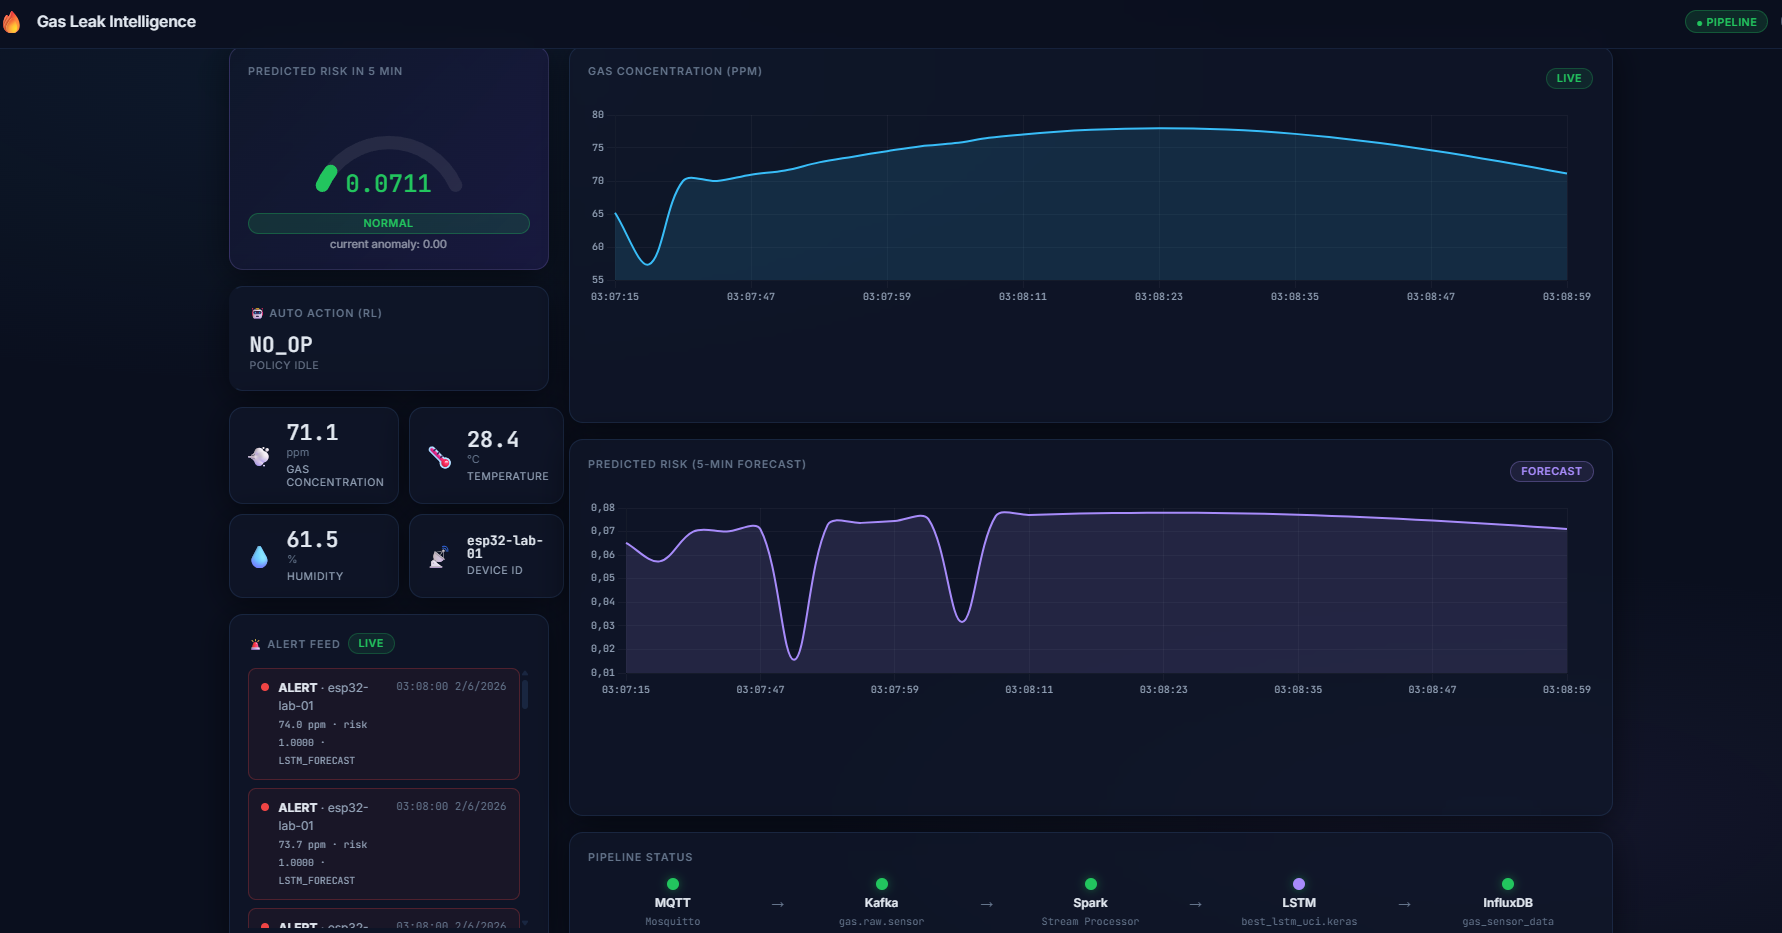
\includegraphics[width=\linewidth]{img/TC1.png}
\captionof{figure}{Kết quả bảng điều khiển của testcase TC1.}
\label{fig:tc1}
\end{minipage}
\end{center}

\begin{center}
\begin{minipage}{0.96\linewidth}
\centering
  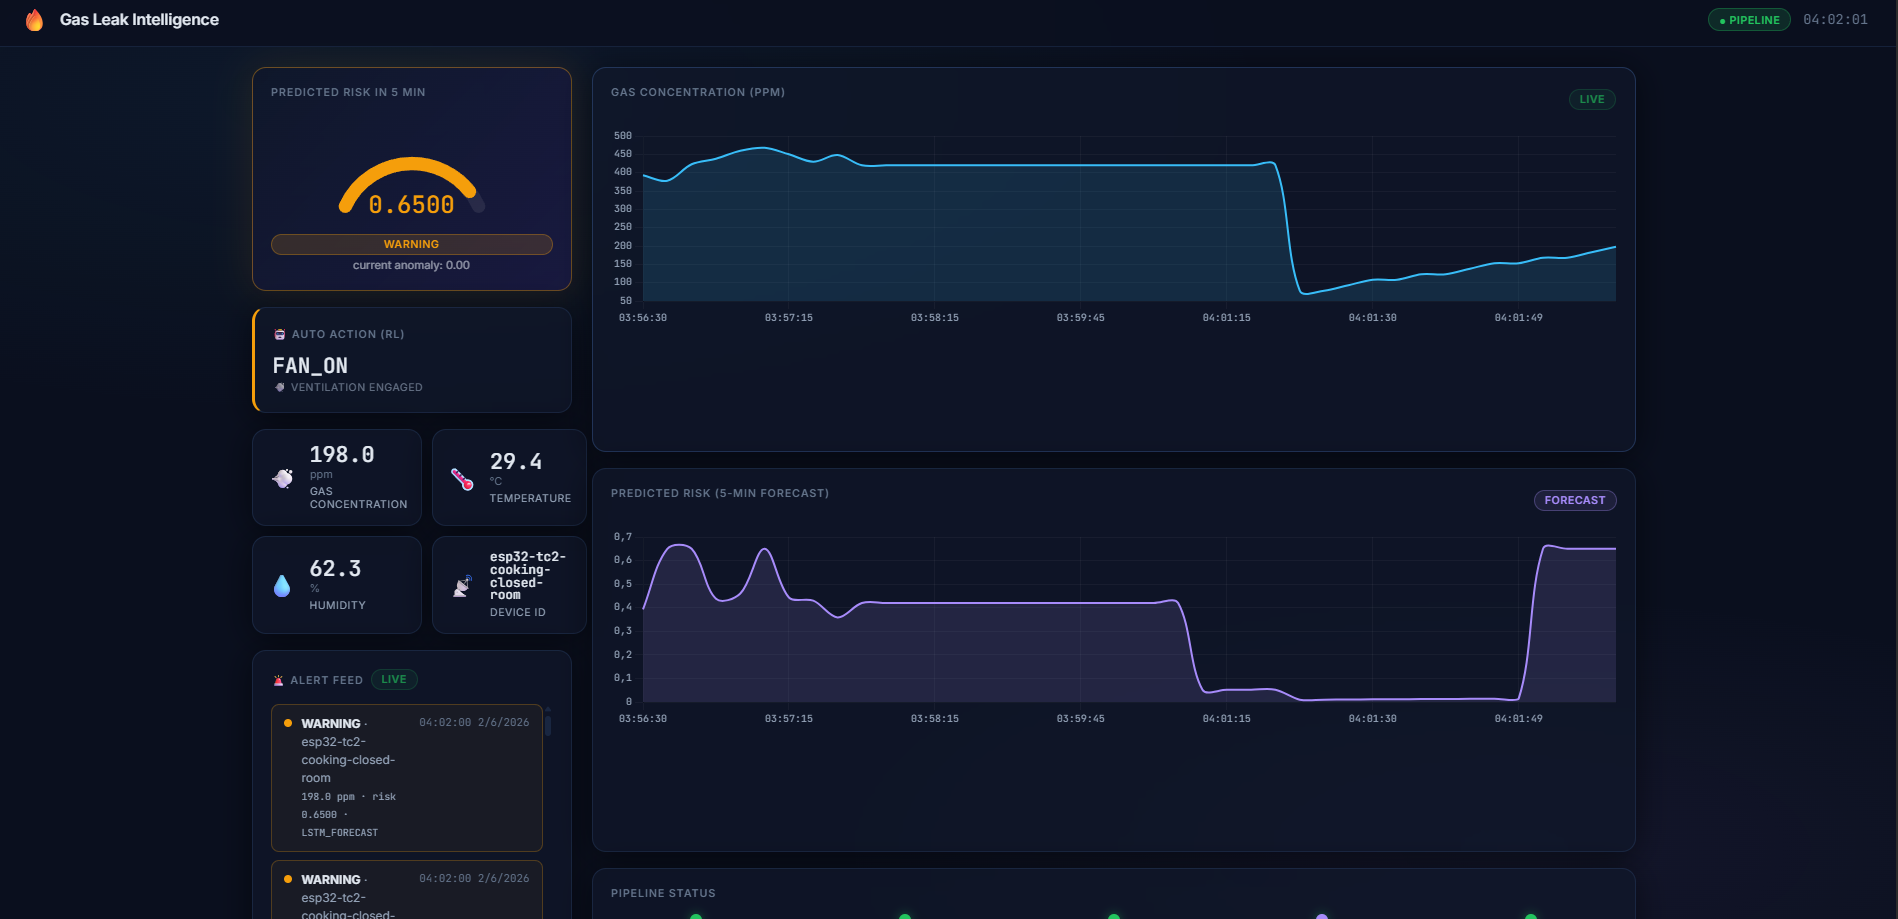
\includegraphics[width=0.48\linewidth]{img/TC2-1.png}
  \hfill
  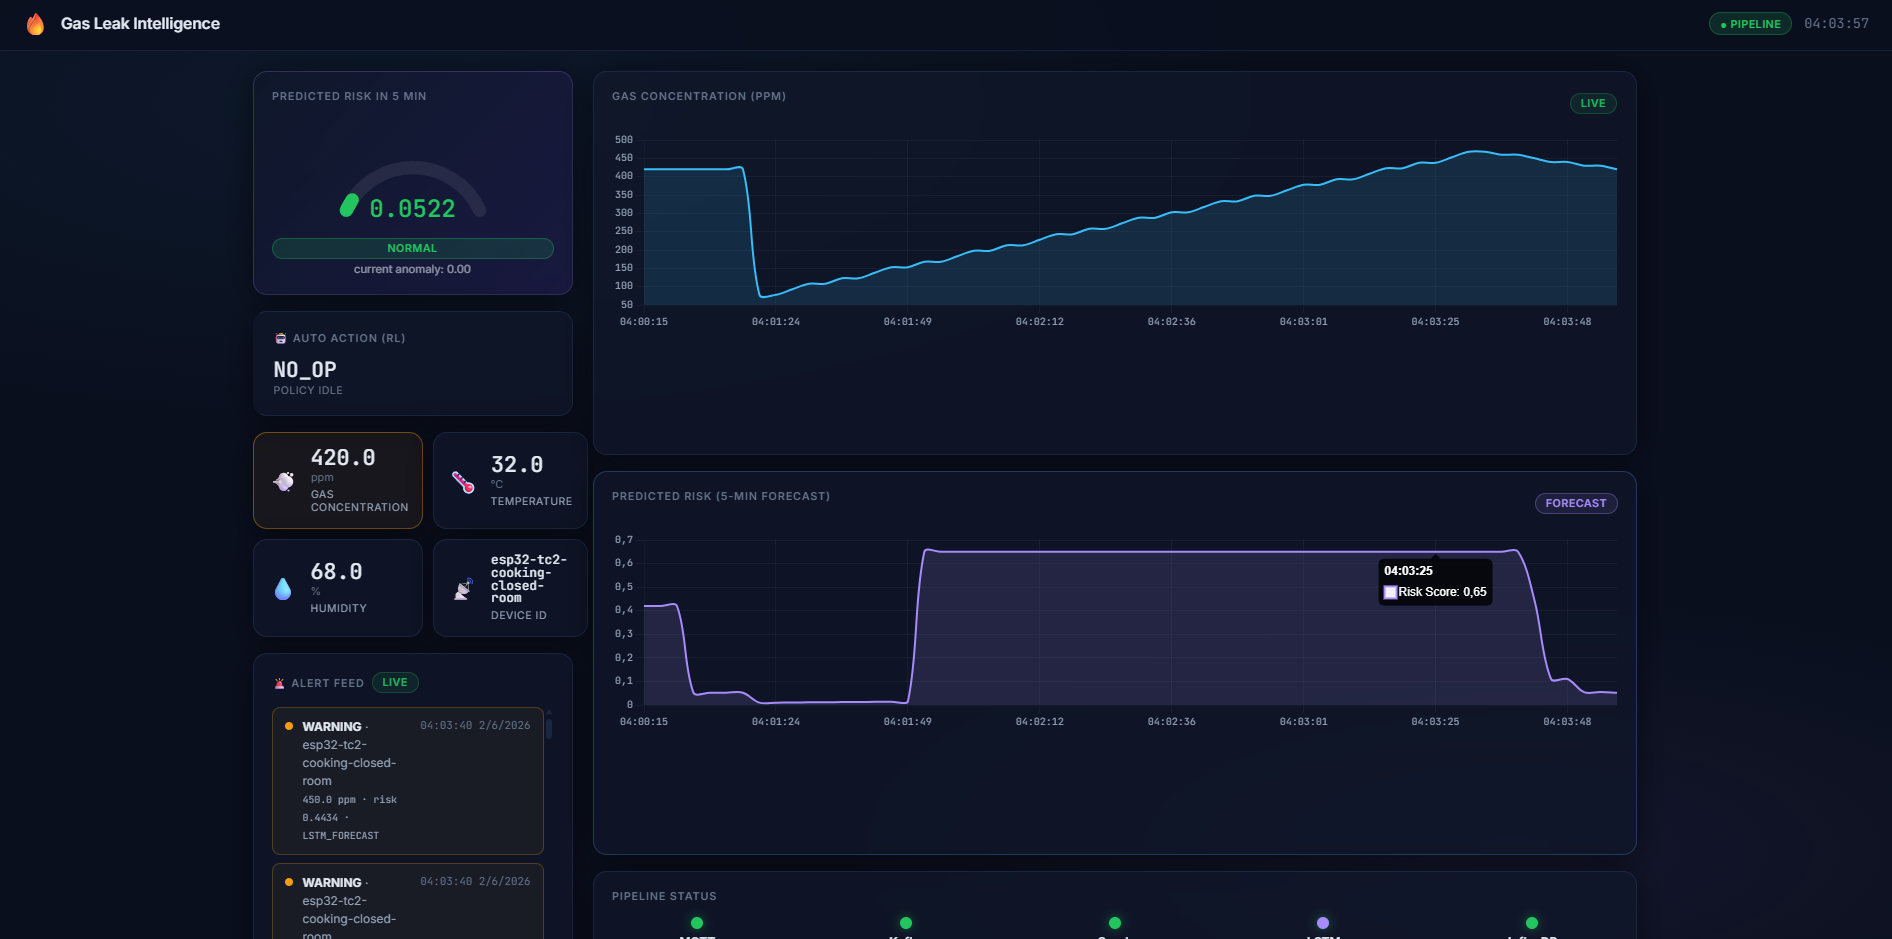
\includegraphics[width=0.48\linewidth]{img/TC2-2.png}

  \captionof{figure}{Kết quả bảng điều khiển của testcase TC2.}
  \label{fig:tc2_result}
\end{minipage}
\end{center}

\begin{center}
\begin{minipage}{0.96\linewidth}
\centering
  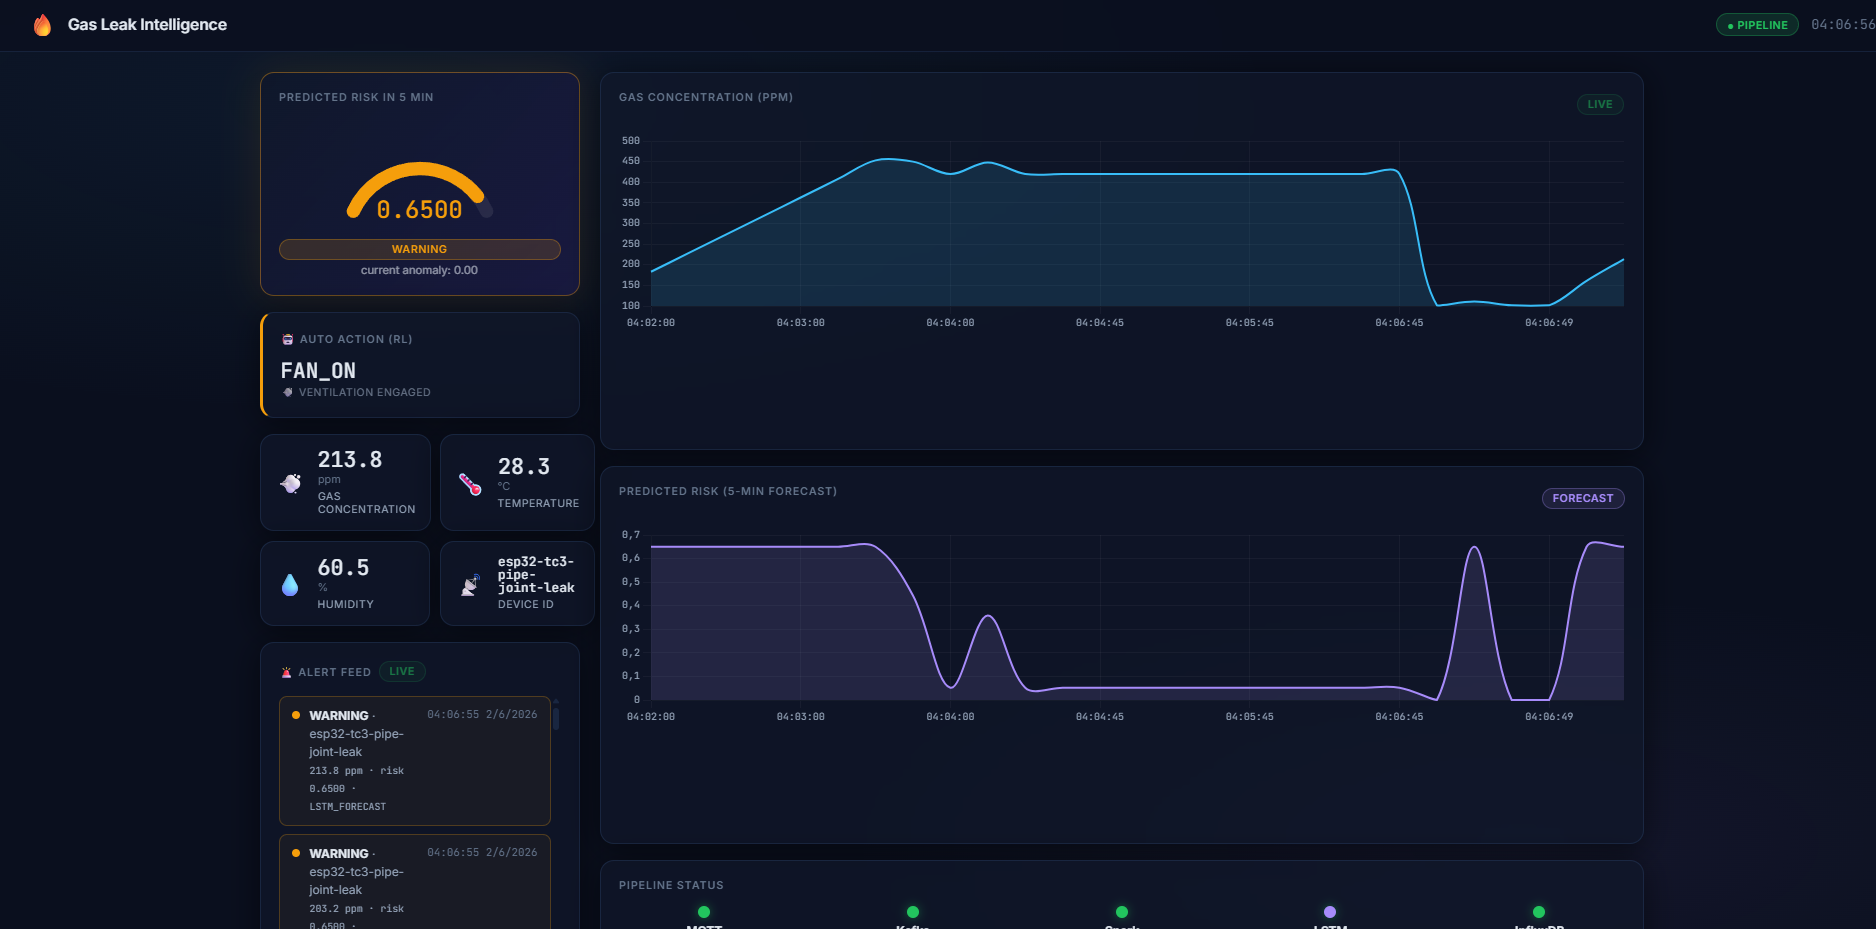
\includegraphics[width=0.48\linewidth]{img/TC3-1.png}
  \hfill
  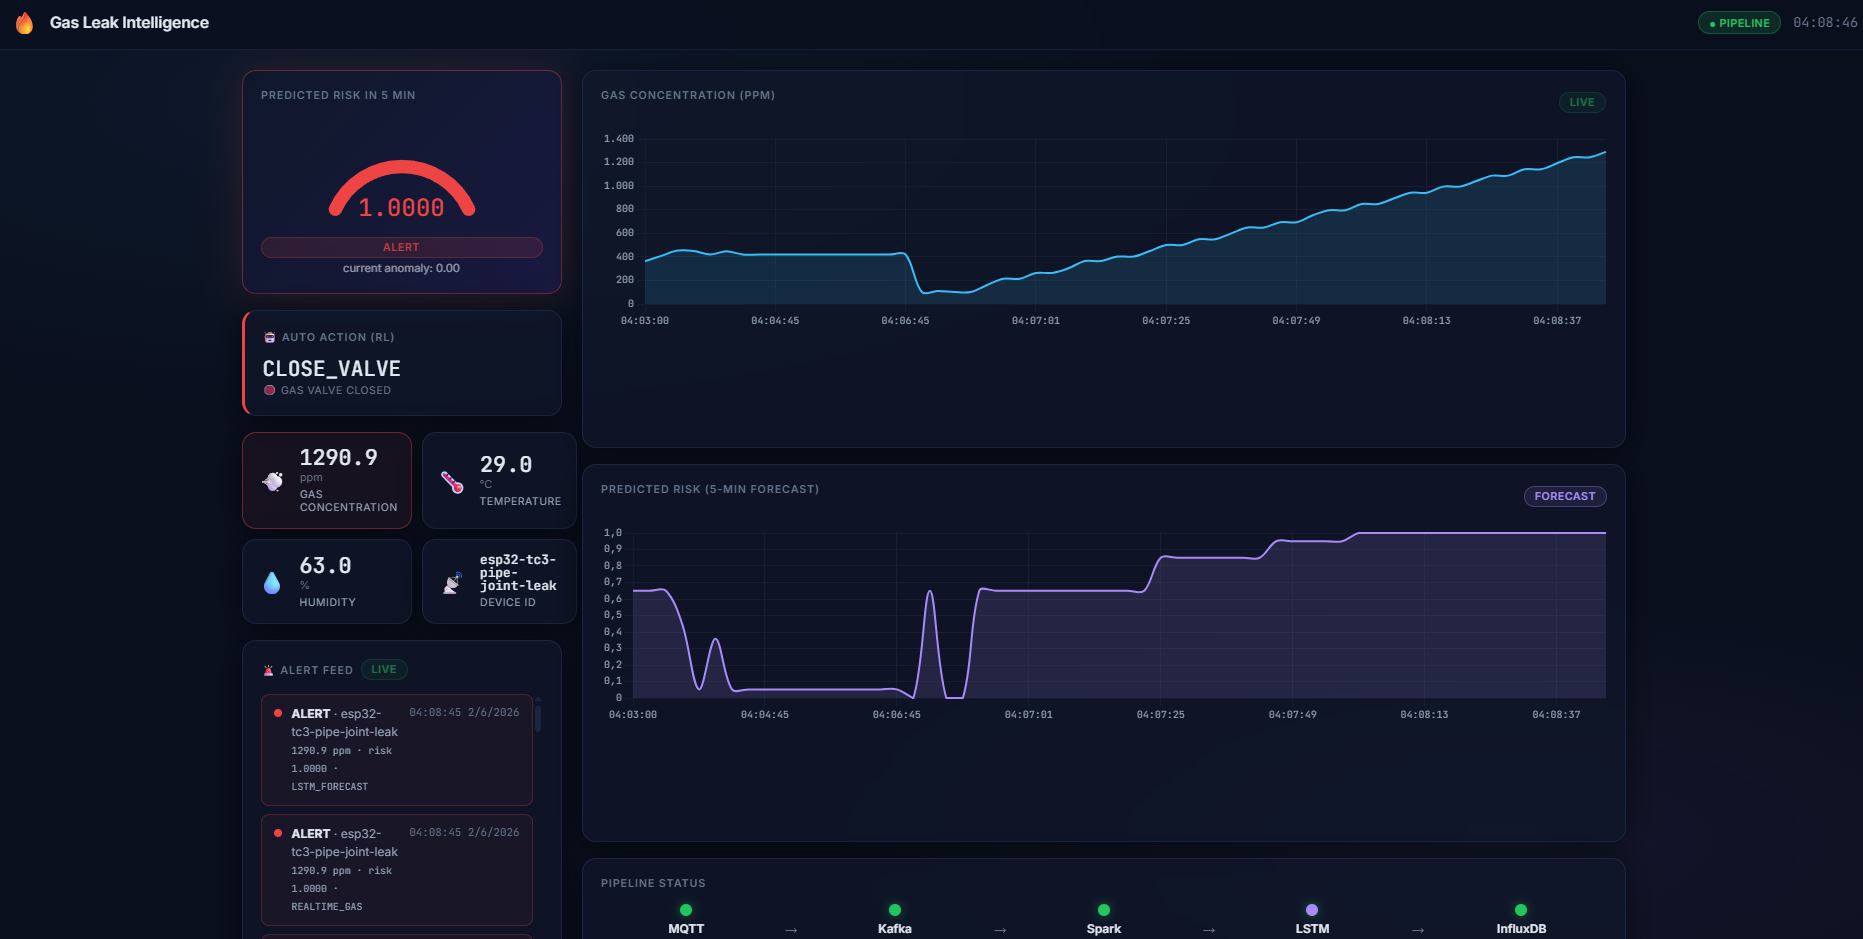
\includegraphics[width=0.48\linewidth]{img/TC3-2.png}

  \captionof{figure}{Kết quả bảng điều khiển của testcase TC3.}
  \label{fig:tc3_result}
\end{minipage}
\end{center}

\begin{center}
\begin{minipage}{0.42\linewidth}
\centering
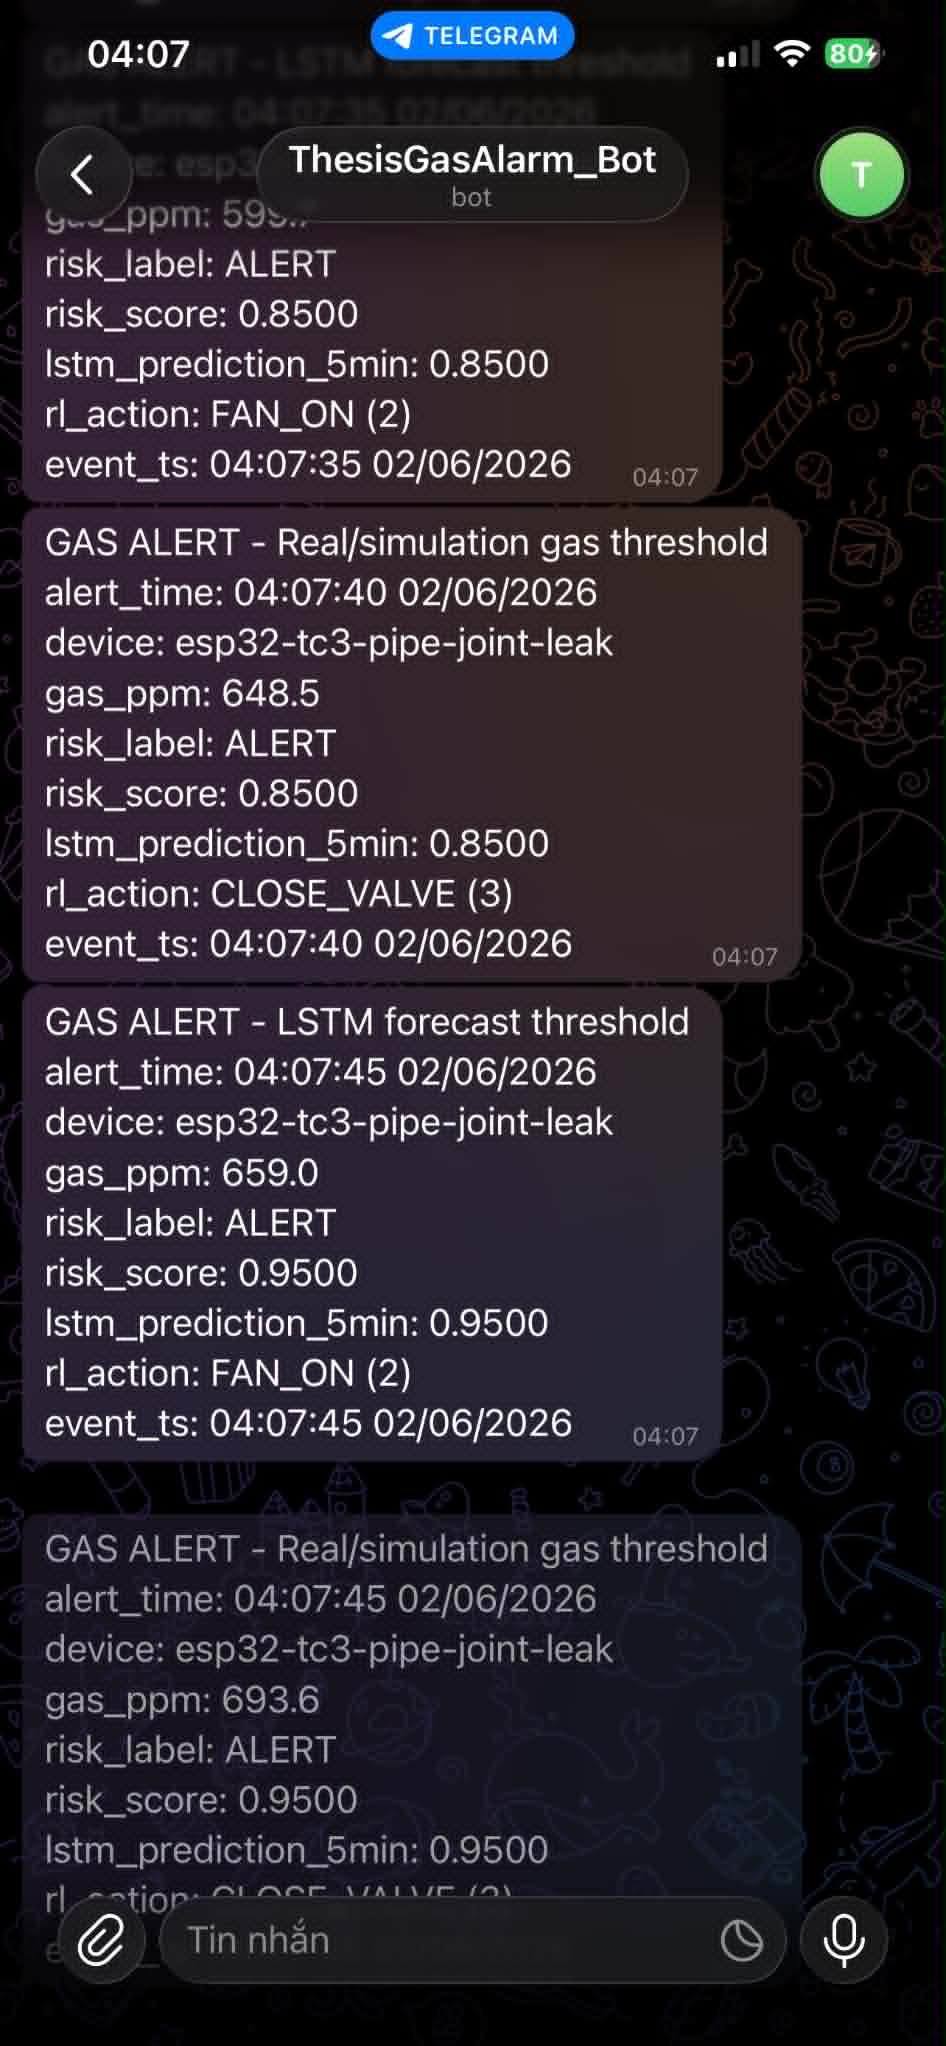
\includegraphics[width=0.82\linewidth]{img/tele_TC3.jpg}
\captionof{figure}{Thông báo Telegram trong testcase TC3.}
\label{fig:tele-tc3}
\end{minipage}
\end{center}

\begin{center}
\begin{minipage}{0.96\linewidth}
\centering
  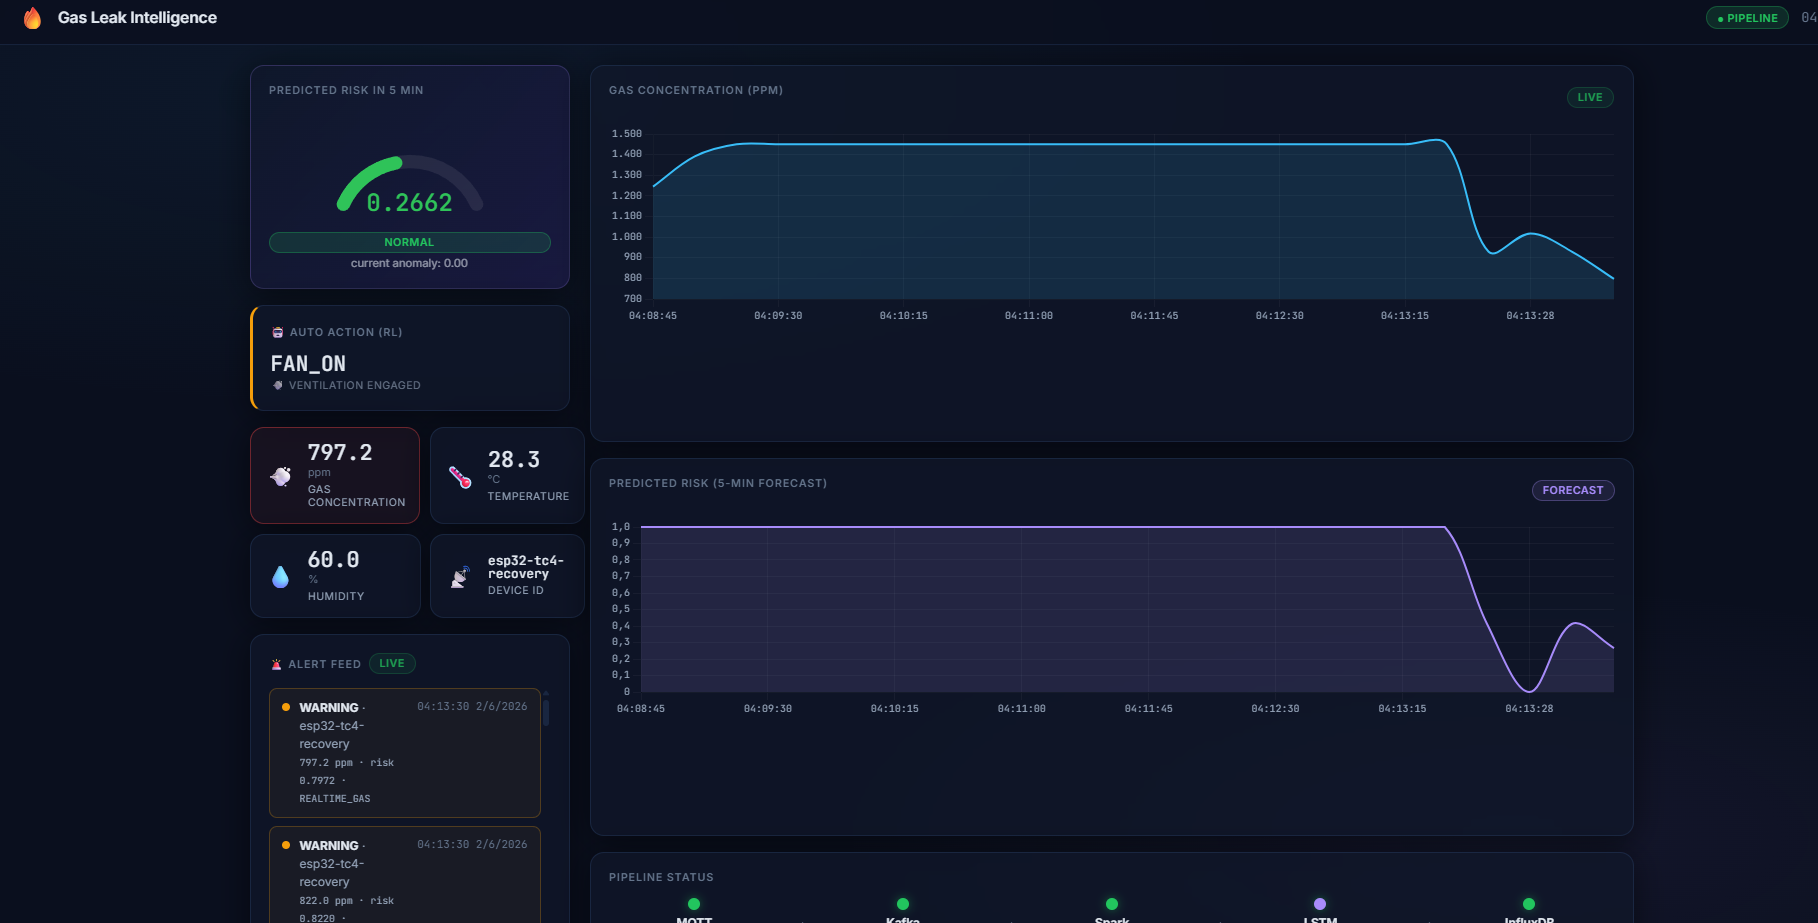
\includegraphics[width=0.48\linewidth]{img/TC4-1.png}
  \hfill
  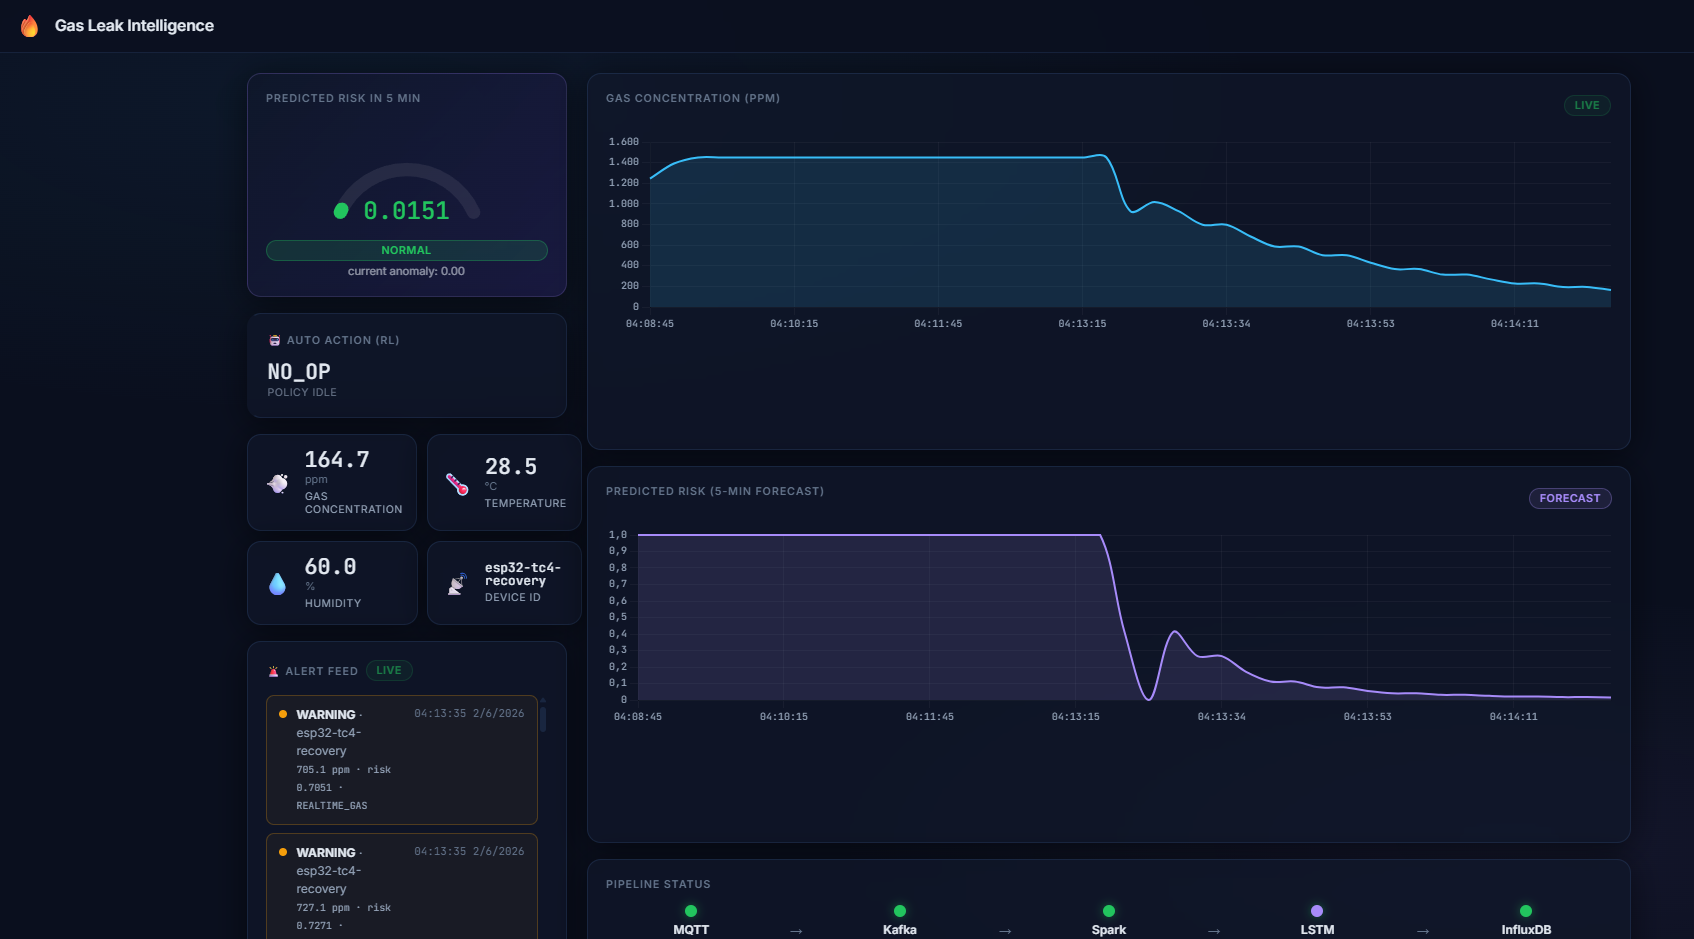
\includegraphics[width=0.48\linewidth]{img/TC4-2.png}

  \captionof{figure}{Kết quả bảng điều khiển của testcase TC4.}
  \label{fig:tc4_result}
\end{minipage}
\end{center}

\begin{center}
\begin{minipage}{0.42\linewidth}
\centering
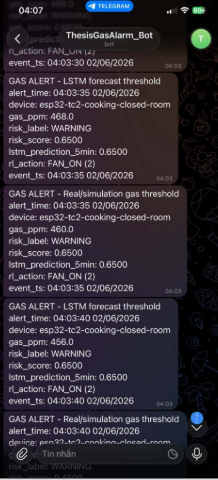
\includegraphics[width=0.82\linewidth]{img/tele-tc4.png}
\captionof{figure}{Thông báo Telegram trong testcase TC4.}
\label{fig:tele-tc4}
\end{minipage}
\end{center}

\subsection{Testcase luồng MQTT--Kafka--Spark}
\label{sec:kafka_pipeline_eval}

\noindent\textbf{a) Mục tiêu đánh giá}

Nhóm testcase luồng xử lý được xây dựng để kiểm tra việc dữ liệu có đi qua đầy đủ các thành phần MQTT, Kafka, Spark và InfluxDB hay không. Đồng thời, phần này cũng làm rõ vai trò của Kafka trong kiến trúc. Khi dữ liệu tăng nhanh hoặc xuất hiện đợt tăng đột biến, Kafka đóng vai trò bộ đệm, giúp tách tốc độ gửi dữ liệu của nguồn phát khỏi tốc độ xử lý của thành phần đọc.

\noindent\textbf{b) Kết quả testcase luồng xử lý}

Kết quả chạy script \texttt{scripts/test/run-kafka-pipeline-tests.ps1} được tổng hợp trong Bảng~\ref{tab:kafka_pipeline_results}.

\begingroup
\small
\renewcommand{\arraystretch}{1.25}
\setlength{\tabcolsep}{4pt}
\setlength{\LTleft}{0pt}
\setlength{\LTright}{0pt}

\begin{longtable}{
  >{\raggedright\arraybackslash}p{2.8cm}
  >{\raggedright\arraybackslash}p{3cm}
  >{\raggedright\arraybackslash}p{3cm}
  >{\raggedright\arraybackslash}p{\dimexpr\textwidth-8.8cm-8\tabcolsep\relax}
}
\caption{Kết quả testcase luồng MQTT--Kafka--Spark}
\label{tab:kafka_pipeline_results} \\
\toprule
\textbf{Testcase} & \textbf{Kafka} & \textbf{Spark/DB} & \textbf{Kết luận} \\
\midrule
\endfirsthead
\toprule
\textbf{Testcase} & \textbf{Kafka} & \textbf{Spark/DB} & \textbf{Kết luận} \\
\midrule
\endhead
\endfoot
\bottomrule
\endlastfoot
TC-P1 Basic & 60/60, 100\% & 60/60, 100\% & Pipeline cơ bản hoạt động đúng. \\
TC-P2 Tải trung bình & 500/500, 100\% & 500/500, 100\% & Ổn định ở tải trung bình, tốc độ gửi khoảng 41 msg/s. \\
TC-P3 Dữ liệu tăng đột biến & 1000/1000, 100\% & 1000/1000, 100\% & Kafka tiếp nhận đủ dữ liệu khi bản tin được gửi nhanh, tốc độ gửi khoảng 646 msg/s. \\
TC-P4 Multi-topic & Raw +5, Alert +6, Action +5 & 5/5 & Các topic raw, alert và action đều có dữ liệu. \\
TC-P5 Invalid data & Recovery 5/5 & Recovery 5/5 & Dữ liệu lỗi không làm bridge/Spark crash; hệ thống tiếp tục xử lý dữ liệu hợp lệ sau đó. \\
\end{longtable}
\endgroup

TC-P1 chứng minh luồng dữ liệu cơ bản hoạt động. TC-P2 cho thấy luồng xử lý vẫn ổn định ở tải trung bình. TC-P3 là testcase quan trọng để chứng minh vai trò bộ đệm của Kafka: dữ liệu được gửi nhanh nhưng Kafka vẫn tiếp nhận đủ bản tin và Spark xử lý dần theo micro-batch. TC-P5 cho thấy hệ thống có khả năng phục hồi khi gặp dữ liệu lỗi.

\begin{center}
\begin{minipage}{0.86\linewidth}
\centering
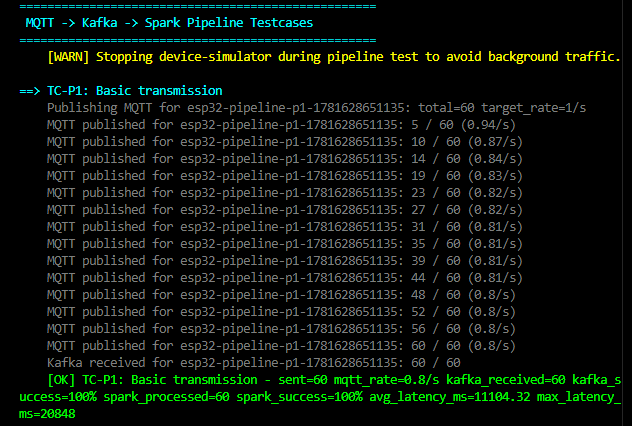
\includegraphics[width=\linewidth]{img/TC-P1.png}
\captionof{figure}{Kết quả kiểm thử luồng xử lý TC-P1.}
\label{fig:TC-P1}
\end{minipage}
\end{center}

\begin{center}
\begin{minipage}{0.86\linewidth}
\centering
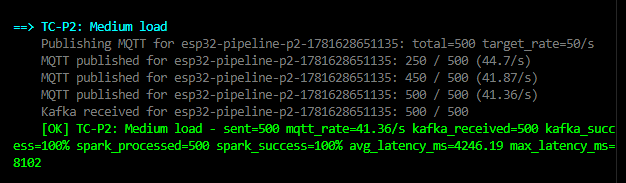
\includegraphics[width=\linewidth]{img/TC-P2.png}
\captionof{figure}{Kết quả kiểm thử luồng xử lý TC-P2.}
\label{fig:TC-P2}
\end{minipage}
\end{center}

\begin{center}
\begin{minipage}{0.86\linewidth}
\centering
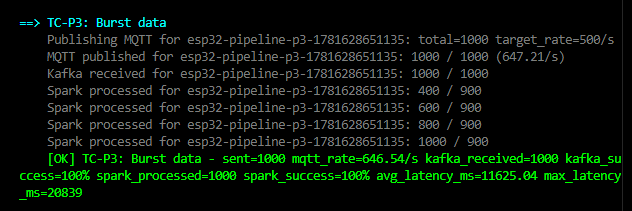
\includegraphics[width=\linewidth]{img/TC-P3.png}
\captionof{figure}{Kết quả kiểm thử luồng xử lý TC-P3.}
\label{fig:TC-P3}
\end{minipage}
\end{center}

\begin{center}
\begin{minipage}{0.86\linewidth}
\centering
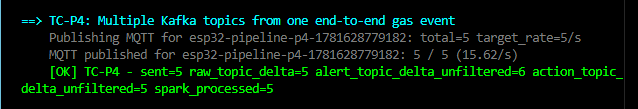
\includegraphics[width=\linewidth]{img/TC-P4.png}
\captionof{figure}{Kết quả kiểm thử luồng xử lý TC-P4.}
\label{fig:TC-P4}
\end{minipage}
\end{center}

\begin{center}
\begin{minipage}{0.86\linewidth}
\centering
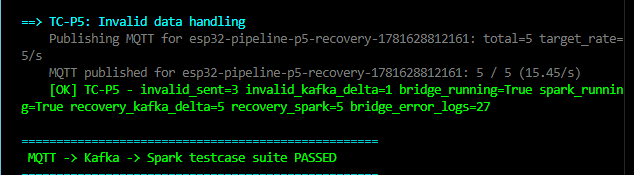
\includegraphics[width=\linewidth]{img/TC-P5.png}
\captionof{figure}{Kết quả kiểm thử luồng xử lý TC-P5.}
\label{fig:TC-P5}
\end{minipage}
\end{center}

\subsection{Độ trễ suy luận LSTM/PPO}
\label{sec:model_latency_eval}

Ngoài độ trễ của luồng xử lý, đề tài đo riêng thời gian suy luận của bộ dự báo LSTM và tác nhân PPO. Kết quả được trình bày trong Bảng~\ref{tab:latency_model}. Trong đó, Mean là độ trễ trung bình, Median là trung vị, P95 là mức mà 95\% mẫu đo nhỏ hơn hoặc bằng giá trị này, và P99 là mức mà 99\% mẫu đo nhỏ hơn hoặc bằng giá trị này. P95/P99 giúp quan sát độ trễ ở phần đuôi phân phối, quan trọng hơn trung bình khi đánh giá hệ thống thời gian thực mềm.

\begingroup
\small
\renewcommand{\arraystretch}{1.25}
\setlength{\tabcolsep}{4pt}
\setlength{\LTleft}{\fill}
\setlength{\LTright}{\fill}

\begin{longtable}{lcccc}
\caption{Độ trễ suy luận mô hình}
\label{tab:latency_model} \\
\toprule
\textbf{Thành phần} & \textbf{Mean} & \textbf{Median} & \textbf{P95} & \textbf{P99} \\
\midrule
\endfirsthead
\toprule
\textbf{Thành phần} & \textbf{Mean} & \textbf{Median} & \textbf{P95} & \textbf{P99} \\
\midrule
\endhead
\endfoot
\bottomrule
\endlastfoot
LSTM bộ dự báo & 76{,}333 ms & 71{,}113 ms & 113{,}650 ms & 136{,}310 ms \\
PPO choose action & 0{,}703 ms & 0{,}690 ms & 0{,}813 ms & 0{,}943 ms \\
\end{longtable}
\endgroup

Kết quả cho thấy LSTM là thành phần tốn thời gian hơn, nhưng độ trễ vài chục mili-giây vẫn nhỏ so với chu kỳ lấy mẫu ở mức giây. PPO gần như không phải nút thắt vì thời gian chọn hành động dưới 1 ms. Vì vậy, độ trễ đầu cuối chủ yếu đến từ micro-batch, I/O và quá trình ghi/đọc cơ sở dữ liệu, không phải từ bộ điều khiển PPO.

\vspace{0.5em}
\noindent\textbf{Kết chương.}

Kết quả đánh giá hệ thống thể hiện qua: mô hình LSTM, bộ điều khiển PPO và luồng triển khai. Kết quả LSTM cho thấy mô hình có khả năng học xu hướng rủi ro từ chuỗi cảm biến theo dạng dự báo sự kiện trong tương lai. Kết quả PPO cho thấy bộ điều khiển có thể giảm \texttt{miss\_rate}, giảm \texttt{peak\_gas} và hạn chế cảnh báo sai tốt hơn các đường cơ sở trong môi trường mô phỏng.

Nhóm testcase kiểm tra kết quả LSTM và PPO TC1--TC4 cho thấy hệ thống phản ứng hợp lý trong các trạng thái bình thường, tăng rủi ro, rò rỉ nguy hiểm và phục hồi. Nhóm testcase luồng xử lý TC-P1--TC-P5 cho thấy Kafka có vai trò rõ ràng trong việc tiếp nhận, đệm và chuyển tiếp dữ liệu cho Spark xử lý. Tóm lại, hệ thống đáp ứng mục tiêu của khóa luận ở mức mô phỏng và tích hợp phần mềm: dữ liệu được xử lý theo thời gian thực, LSTM cung cấp tín hiệu dự báo, PPO lựa chọn hành động điều khiển, còn bảng điều khiển và Telegram hỗ trợ hiển thị/cảnh báo cho người dùng.
